\chapter{BT Studio: avances}\label{cap:bt-studio-avances}

En este capítulo, se detallarán los avances y contribuciones realizadas en este TFG a la herramienta de BT Studio. Se hablará sobre las mejoras y cambios de sus componentes, así como las implicaciones de estos para la experiencia del usuario.

Todas las siguientes modificaciones han sido realizadas con los fundamentos de BT Studio, definidos en el capítulo \ref{cap:bt-studio}. Estas han mejorado la implementación de esos fundamentos en la herramienta añadiendo funcionalidades adicionales. También se han producido más cambios en la herramienta como parte de un proyecto de GSOC \footnote{\url{https://theroboticsclub.github.io/gsoc2024-Oscar_Martinez/}} centrado en la composición de árboles de comportamiento, externo pero muy relacionado con este TFG.

Todos estos cambios han sido realizados en los siguientes repositorios de GitHub:

\begin{itemize}
    \item \textbf{bt-studio}: \url{https://github.com/JdeRobot/bt-studio}.
    \item \textbf{RoboticsInfrastructure}: \url{https://github.com/JdeRobot/RoboticsInfrastructure}.
    \item \textbf{RoboticsApplicationManager}: \url{https://github.com/JdeRobot/RoboticsApplicationManager}.
    \item \textbf{unibotics-webserver}: es privado.
    \item \textbf{RoboticsBackend}: es privado.
\end{itemize}

\section{Modificaciones al diseño}\label{sec:mod-design}

Para permitir añadir nuevas funcionalidades, ha sido necesario realizar varios cambios en el diseño de la estructura de BT Studio. Estos cambios se van a explicar en más detalle en los siguientes apartados:

\begin{figure}[H]
    \centering
    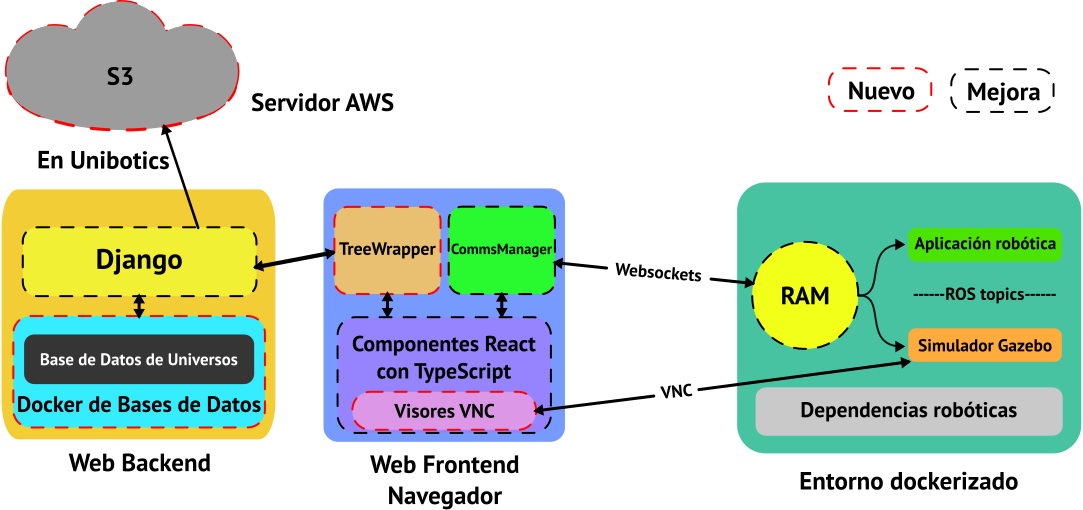
\includegraphics[width=\textwidth]{figures/bt-avances/bt-structure.png}
    \caption{Diseño de la estructura de BT Studio}
    \label{fig:bt-new-struct}
\end{figure}

\subsection{Estructura de un proyecto robótico}

La estructura de un proyecto robótico cualquiera en BT Studio ha sufrido bastantes cambios para poder adaptarse a la inclusión de los universos y permitir una mayor generalización de estos proyectos.

Partiendo de la estructura definida en \ref{sec:bt-struct-old}, se han modificado los siguientes puntos:

\begin{itemize}
    \item División de un proyecto en dos directorios principales: \textit{code} (contiene el código de la aplicación robótica, es decir, sus acciones y su árbol/subárboles) y \textit{universes} (incluye los universos definidos para ese proyecto, que son la combinación de un escenario simulado y un modelo de robot). Además, también se añade el fichero de configuración del proyecto explicado en el apartado a continuación.
    \item Traslado del fichero JSON que guarda el árbol de comportamiento principal al directorio \textit{trees} que se encuentra dentro de \textit{code}. Dentro de este directorio también se alojan los subárboles de comportamiento.
    \item Renombrado el fichero JSON que guarda el árbol de comportamiento principal de \textit{graph.json} a \textit{main.json}.
    \item Incorporación de los universos, que serán explicados con más detalle en la sección \textit{universos}.
\end{itemize}

\begin{figure}[H]
    \centering
    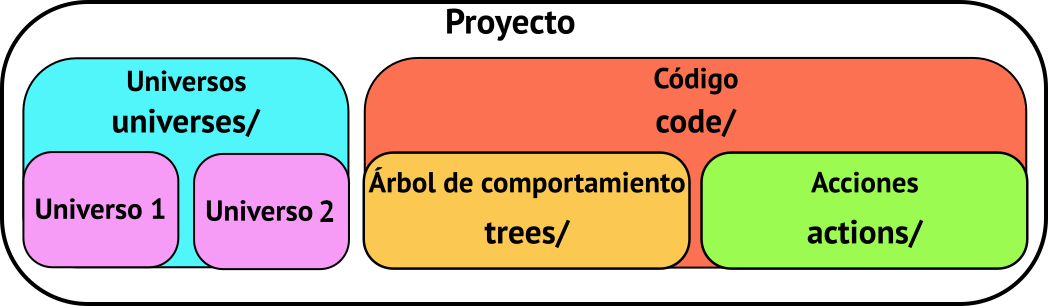
\includegraphics[width=0.7\textwidth]{figures/bt-avances/bt-proy-new.png}
    \caption{Estructura nueva de un proyecto de BT Studio}
    \label{fig:estructura-nueva}
\end{figure}

\subsection{Personalización y configuración}\label{sec:config}

Con el objetivo de permitir al usuario personalizar diferentes aspectos del web IDE, se ha añadido la posibilidad de configurar cada proyecto individualmente. Para conseguir esto, se añadió un fichero JSON extra a la estructura de los proyectos con el fin de guardar la configuración de estos de forma sencilla. Los puntos que pueden ser configurados son los siguientes:

\begin{itemize}
    \item \textbf{theme:} apariencia de BT Studio, permitiendo cambiar entre modo oscuro (\textit{dark}) y claro (\textit{light}).
    \item \textbf{btOrder:} orden de ejecución del árbol de comportamiento. Puede ser de arriba hacia abajo (\textit{top-to-bottom}) o viceversa (\textit{bottom-to-top}).
    \item \textbf{editorShowAccentColors:} mostrar los colores de las acciones en el navegador de ficheros, más detalle en la sección \textit{navegador de ficheros}. Puede ser verdadero (\textit{true}) o falso (\textit{false}).
\end{itemize}

Por otra parte, para permitir al usuario su modificación se han creado un modal en el frontend web y dos funciones en el backend web.

\subsubsection{Frontend}

Empezando por el frontend, primero se debe definir la forma de uso de estas opciones por toda la aplicación. Para esto se ha empleado un elemento de React llamado \textit{context} \footnote{\url{https://react.dev/learn/passing-data-deeply-with-context}}. Este elemento es usado como una alternativa a pasar \textit{props} y que suele ser utilizado cuando un componente React debe pasar información, ya sean funciones o variables, a un gran número de componentes que se encuentran varios niveles más abajo, lo que permite usar estos datos sin tener que pasarlos de forma explícita.

Este \textit{context} se ha usado para crear en el fichero \textit{frontend/src/components/options/Options.tsx} el contexto usando el método de React \textit{createContext} y para crear un componente que va a proveer ese contexto al resto de la aplicación, \textit{OptionsProvider}. Este componente se encarga de encapsular el contexto y las funciones necesarias para modificar las configuraciones que este provee.

Con el proveedor ya creado hace falta añadirlo en la aplicación para que se pueda acceder al contexto. Se añade \textit{OptionsProvider} a BT Studio en el fichero \textit{frontend/src/index.js} para que esté disponible para todos los componentes, que accederán al contexto usando la función \textit{useContext} de React pasándole como parámetro el contexto defindo en \textit{frontend/src/components/options/Options.tsx}.

Ahora que ya está definida la forma de modificar la configuración, nos podemos centrar en la interfaz que usará el usuario para personalizar el proyecto. Para ello se crea el componente \textit{SettingsModal} definido en \textit{frontend/src/components/settings\_popup/SettingsModal.tsx}. En este se muestran las distintas posibles configuraciones en forma de lista, que está dividida en diferentes secciones para indicar el tipo de configuración.

\begin{figure}[H]
    \centering
    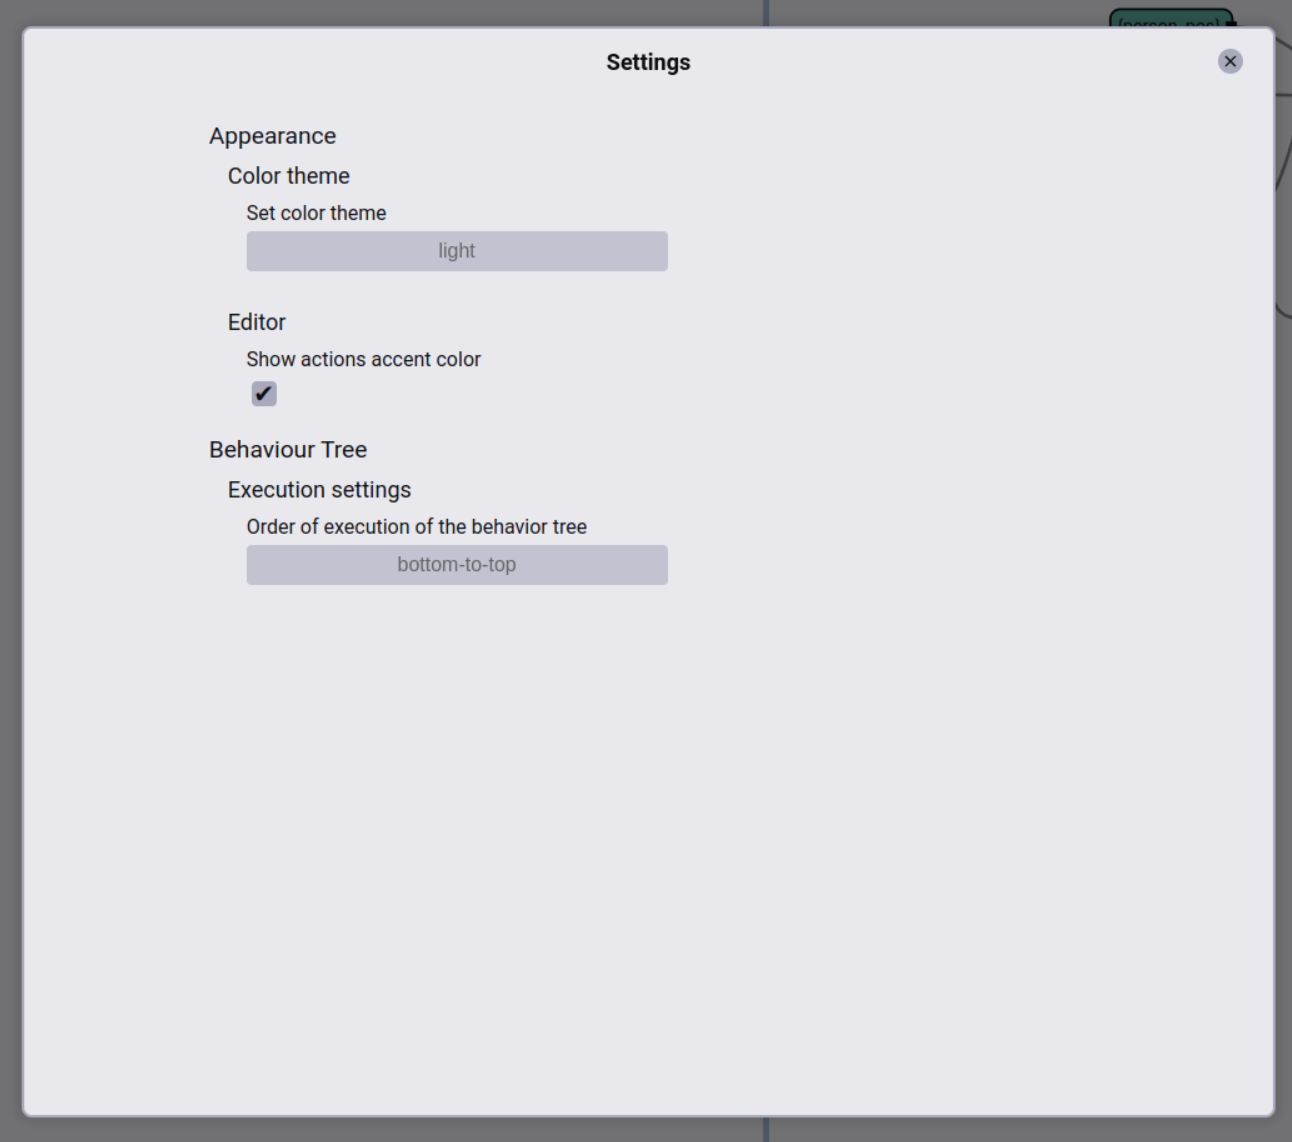
\includegraphics[width=0.5\textwidth]{figures/bt-avances/setting-light.png}
    \caption{Modal de configuración en modo claro de BT Studio}
    \label{fig:ejemplo}
\end{figure}

Cada una de las entradas de los diferentes aspectos de configuración modificar se encuentra estructurada de la misma manera:

\begin{itemize}
    \item Título: muestra dónde se produce el cambio y lo que hace de forma muy resumida.
    \item Descripción: describe de forma más detallada el objetivo de esa configuración.
    \item Configuración: permite editar la configuración. Es una casilla de verificación para aquellas que sus posibles valores son verdadero o falso, y una lista desplegable con los posibles valores para las que tienen múltiples valores definidos previamente.
\end{itemize}

Todas las partes de la estructura anterior están creadas en distintos componentes que se pueden encontrar dentro de los directorios \textit{frontend/src/components/settings\_popup/sections}, para las diferentes secciones, y \textit{frontend/src/components/settings\_popup/options}, para los diferentes tipos de configuraciones. 

\subsubsection{Backend}

Y por último, en la parte del backend se han creado dos funciones nuevas: \textit{save\_project\_configuration} y \textit{get\_project\_configuration}. La primera sirve para guardar los cambios en la configuración y la segunda para devolver el contenido de esta al frontend.

El fichero de configuración está guardado con el formato JSON y con el nombre \textit{config.json}. Un ejemplo de uno de estos ficheros para un proyecto llamado \textbf{MiProyecto} sería:

\lstinputlisting[
    float,
    floatplacement=!htp,
    language=json,
    caption=Ejemplo de un fichero de configuración de un proyecto en BT Studio
]{code/config.json}

\subsection{Estructura de la plataforma}

La estructura de la plataforma ha sufrido unos pequeños cambios en el proceso de generación de aplicaciones, ya que este no era el adecuado de cara a la integración en la plataforma web Unibotics. Esto último se tratará más detalladamente en la sección \ref{sec:bt-unib}.

Los cambios se pueden resumir en la incorporación de un paso intermedio entre la traducción de la aplicación robótica y el ejecutable de la misma. Este paso consiste en el empaquetado de la aplicación y, añadiendo los ficheros necesarios al resultante de la traducción para que se pueda ejecutar en el entorno dockerizado del Robotics Backend o en un entorno local y comprimirlos en forma de archivo ZIP.

\begin{figure}[H]
    \centering
    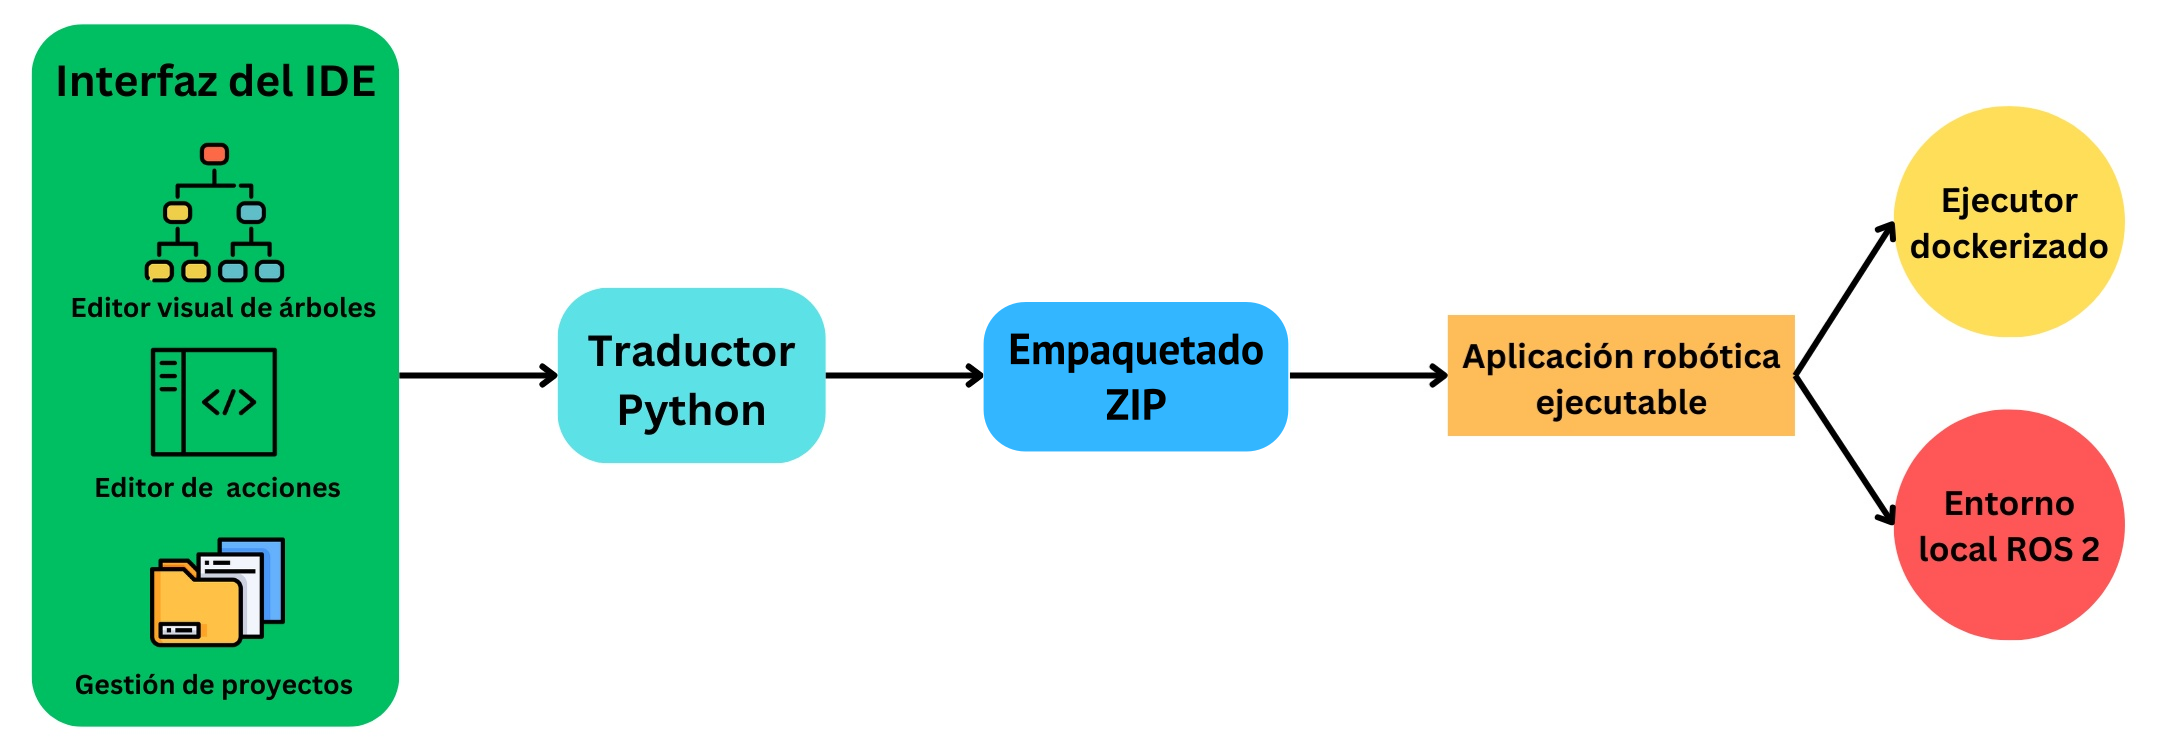
\includegraphics[width=\textwidth]{figures/bt-avances/flow.png}
    \caption{Proceso de generación de aplicaciones en BT Studio}
    \label{fig:ejemplo-23}
\end{figure}

\subsection{Uso exclusivo de TypeScript}

BT Studio estaba compuesto por una mezcla de JavaScript y TypeScript anteriormente. Esto causaba que a veces, por culpa de la naturaleza no tipada de JS, se produjeran errores en ejecución al volverse una variable un tipo no esperado como \textit{null} o \textit{undefined}. Para solucionar todos estos casos se ha migrado todo el código a TS, lo que además ha mejorado la legibilidad y la comprensión del código escrito.

Además, en las partes donde se usaba TS se ha reemplazado todas las definiciones de \textit{any}, que causaban que no se comprobara el tipo, por tipos estrictos.

\subsection{Comunicación con el backend web}

La forma de comunicarse con la API del backend web desde el frontend web ha sido estandarizada y trasladada a un solo fichero de TypeScript llamado \textit{frontend/src/api\_helper/TreeWrapper.ts}.

Anteriormente, esta comunicación usaba tanto el paquete de \textit{axios} \footnote{\url{https://www.npmjs.com/package/axios}} como la función estándar de \textit{fetch} dependiendo del componente, lo que hacía que hubiera múltiples problemas a la hora de modificar una de las funciones del backend dado el distinto funcionamiento de las dos maneras. Para solucionar esto se han sustituido todas las instancias donde se usaba \textit{fetch} por \textit{axios} y se han abstraído todas las llamadas al backend en funciones de TS.

El abstraer y unificar esta comunicación mejora considerablemente el mantenimiento de la aplicación, así como la expansión de la misma.

\subsection{Uso de BT Studio}\label{sec:uso-bt}

Por último, el uso de BT Studio tanto para desarrolladores como usuarios ha cambiado drásticamente. Antes de estas mejoras era necesario la instalación en local del repositorio de BT Studio, así como la de múltiples dependencias como: NPM, Django, yarn, Node.js, múltiples paquetes de Python y múltiples paquetes de JavaScript. Esto, junto con la necesidad de que algunas de estas dependencias necesitaran una versión específica, causaba un gran número de problemas a la hora de instalar y usar BT Studio.

Para solucionarlo, ahora el uso como usuario es enteramente con un contenedor docker (y de forma mixta, Docker y local, para los desarrolladores). Siguiendo el ejemplo de Robotics Academy (se puede considerar la versión offline de Unibotics) se usa una imagen de docker que contiene el Robotics Backend y la aplicación, en este caso BT Studio. Esto permite a los usuarios poder usarlo sin necesidad de descargar el repositorio de BT Studio, ni ninguna dependencia, a excepción de docker, y simplifica su uso a un simple comando.

\lstinputlisting[
    float,
    floatplacement=!htp,
    language=bash,
    label=cod:user\_launch\_BT-Studio,
    caption=Comando para lanzar BT Studio como usuario
]{code/launch-user.txt}

Para los desarrolladores también se simplifica bastante, pero aun así hay una mayor complejidad. Para estos hay que hablar de dos puntos diferentes: el BTDI o BT Studio Docker Image y el script de desarrollador. Para poder acceder a BT Studio usando estos habrá que ir a la dirección \textit{http://0.0.0.0:7164} en el navegador.

\subsubsection{BT Studio Docker Image}

El objetivo de esta imagen docker es permitir al desarrollador crear una imagen de BT Studio igual que las oficiales pero usando las ramas deseadas por este. Esto permite la personalización de la composición del Robotics Backend, es decir, elegir las ramas de Robotics Infrastructure y de Robotics Application Manager.

Todo esto viene empaquetado dentro del script \textit{build.sh} hallado en el directorio \textit{scripts/BTDI}, para una mejor experiencia de uso.

Más información sobre esto en la sección \textit{Ejecución dockerizada} más adelante.

\subsubsection{Script de lanzamiento para desarrolladores}

Para finalizar, ahora que el desarrollador posee la capacidad de crear imágenes docker de BT Studio personalizadas, podemos usar un método similar al usado por los usuarios para lanzar BT Studio. En este caso se utiliza el script llamado \textit{develop.sh} encontrado en el directorio \textit{scripts}.

Este instala las dependencias faltantes, compila el frontend y lanza los contenedores docker usando la herramienta docker-compose explicada en el capítulo \ref{cap:tecnologias}. Esta lanza dos contenedores, uno con las bases de datos correspondientes a los universos, se explicará más detalladamente en la sección \textit{universos}, y otro con la imagen docker oficial de BT Studio o una definida por el desarrollador. La peculiaridad de estos contenedores, es que gracias a docker, se cambia el contenido de las bases de datos de universos y BT Studio por sus contrapartes que se encuentran en local, permitiendo probar las modificaciones a la herramienta de la misma manera que anteriormente.

\section{Backend web del IDE BT Studio}

El backend ha sufrido una ampliación del API para proporcionar no solo una interfaz para la gestión de proyectos, archivos y generación de aplicaciones, sino también para la gestión de universos. En esta sección se explicarán las mejoras realizadas a las funciones ya existentes y las nuevas funciones añadidas para soportar las funcionalidades añadidas en el frontend que estarán explicadas en la próxima sección. 

\subsection{Mejoras}

La funcionalidad básica encargada de la generación de aplicaciones ha sido modificada para permitir que la escalabilidad dentro de la plataforma de Unibotics sea mejor, ya que reduce la cantidad de cómputo en el servidor. Esto se tratará con más detalle en su propia sección, la \textit{integración con Unibotics}, junto con el resto de modificaciones específicas para esa plataforma.

Las modificaciones al resto de funciones serán mostradas en la siguiente lista junto con el nombre de la función en el backend:

\begin{itemize}
    \item \textbf{create\_project:} añadido soporte para la nueva estructura de los proyectos explicada anteriormente.
    \item \textbf{get\_project\_list:} no ha sufrido modificaciones.
    \item \textbf{save\_project\_graph:} renombrado a \textbf{save\_base\_tree} y adaptado a la nueva estructura de los proyectos. 
    \item \textbf{get\_project\_graph:} adaptado a la nueva estructura de los proyectos.
    \item \textbf{get\_file\_list:} cambio en la forma de enumerar los archivos para adecuarse al nuevo navegador de ficheros que se explicará en la siguiente sección. 
    \item \textbf{get\_file:} adaptado a la nueva estructura de los proyectos.
    \item \textbf{create\_file:} adaptado a la nueva estructura de los proyectos y a las nuevas funcionalidades del nuevo navegador de ficheros.
    \item \textbf{delete\_file:} adaptado a la nueva estructura de los proyectos.
    \item \textbf{save\_file:} adaptado a la nueva estructura de los proyectos.
    \item \textbf{generate\_app:} renombrado a \textbf{generate\_local\_app}. Reimplementación completa para adecuarlo a su uso en Unibotics, esto será explicado con más detalle en un apartado de la sección \textit{ejecución dockerizada}.
    \item \textbf{get\_dockerized\_app:} reimplementación completa para adecuarlo a su uso en Unibotics, esto será explicado con más detalle en la sección \textit{ejecución dockerizada}.
\end{itemize}

\subsection{Novedades}

Al igual que se han modificado la mayoría de las funciones antiguas para adaptarse a las novedades del frontend, también se han añadido nuevas funciones. Estas adiciones están estrechamente relacionadas con sus contrapartes en el frontend y la mayoría se explicarán en más detalle en sus respectivas secciones o apartados más adelante.

La lista de las funciones añadidas al backend es la siguiente:

\begin{itemize}
    \item \textbf{save\_project\_configuration:} guarda la configuración del proyecto actualizada.
    \item \textbf{get\_project\_configuration:} devuelve la configuración del proyecto.
    \item \textbf{delete\_project:} permite eliminar un proyecto existente, borrando todos los ficheros incluidos dentro de este.
    \item \textbf{upload\_universe:} permite subir un universo propio del usuario en forma de fichero ZIP, además genera los directorios y la configuración necesaria.
    \item \textbf{add\_docker\_universe:} crea un nuevo universo usando los disponibles en el Robotics Backend, además genera los directorios y la configuración necesaria.
    \item \textbf{delete\_universe:} elimina un universo existente, borrando todos los ficheros incluidos dentro de este.
    \item \textbf{get\_universes\_list:} enumera todos los universos existentes.
    \item \textbf{get\_universe\_zip:} genera un archivo ZIP con todos los ficheros necesarios para el lanzamiento del universo en el Robotics Backend. Esto solo está disponible para los universos que no son del Robotics Backend.
    \item \textbf{get\_universe\_configuration:} devuelve la configuración del universo correspondiente.
    \item \textbf{list\_docker\_universes:} devuelve una lista de todos los universos disponibles en el Robotics Backend, permitiendo al usuario seleccionar el universo deseado. Usa la base de datos de universos para mostrar esta información.
    \item \textbf{get\_docker\_universe\_path:} devuelve información adicional sobre el universo, si este está disponible en el Robotics Backend. Usa la base de datos de universos para mostrar esta información.
    \item \textbf{get\_tree\_structure:} devuelve la estructura básica del árbol de comportamiento que será usada en el monitor de ejecución.
    \item \textbf{get\_subtree\_structure:} devuelve la estructura básica del subárbol de comportamiento que será usada en el monitor de ejecución.
    \item \textbf{rename\_file:} permite renombrar un archivo.
    \item \textbf{create\_folder:} crea un nuevo directorio vacío en la ubicación especificada en el nuevo navegador de ficheros.
    \item \textbf{rename\_folder:} permite renombrar un directorio.
    \item \textbf{delete\_folder:} elimina un directorio específico y todos sus contenidos.
    \item \textbf{upload\_code:} permite subir múltiples ficheros comprimidos en un solo archivo ZIP en la ubicación especificada en el nuevo navegador de ficheros.
    \item \textbf{create\_action:} permite crear el archivo necesario para una nueva acción a partir de diferentes plantillas, que son especificadas en el nuevo modal de creación de acciones.
    \item \textbf{get\_actions\_list:} enumera todas las acciones existentes.
\end{itemize}

\subsection{Mejoras en el traductor}

Por último, también se ha introducido una mejora en el traductor de JSON a XML. Para poder aplicar de manera correcta las dos variantes en el orden de ejecución del árbol de comportamiento introducido en el apartado \ref{sec:config} ha hecho falta añadir al traductor la capacidad de ordenar los nodos por la altura a la que se encuentran en el diagrama. Esto permite que varios nodos pertenecientes a la misma profundidad del árbol se ordenen de forma correcta para su traducción a XML.

\section{Frontend web del IDE BT Studio}\label{sec:bt-frontend}

En esta sección se va a hablar sobre las mejoras realizadas en el frontend de BT Studio. Estas no tienen que afectar exclusivamente a la experiencia del usuario, sino que también se centran en la mejora de la organización del frontend.

A todos los cambios que se van a presentar a continuación hay que sumarle aquellos presentados en la sección \ref{sec:mod-design}, como la creación de configuraciones, el uso de TypeScript o la mejora de la comunicación con el backend web. A estos se añaden los que van a ser explicados en sus secciones particulares, como el navegador de archivos, el modal de universos o el monitor de ejecución.

Dicho esto, las mejoras y adiciones que se van a presentar a continuación mezclarán los modos gráficos claros y oscuros de manera aleatoria donde haya imágenes disponibles.

También se ha modificado el icono de la asociación de JdeRobot por el icono de Unibotics solo en la versión \textit{online}, que además devuelve al usuario a la página de inicio de Unibotics.

\begin{figure}[H]
    \centering
    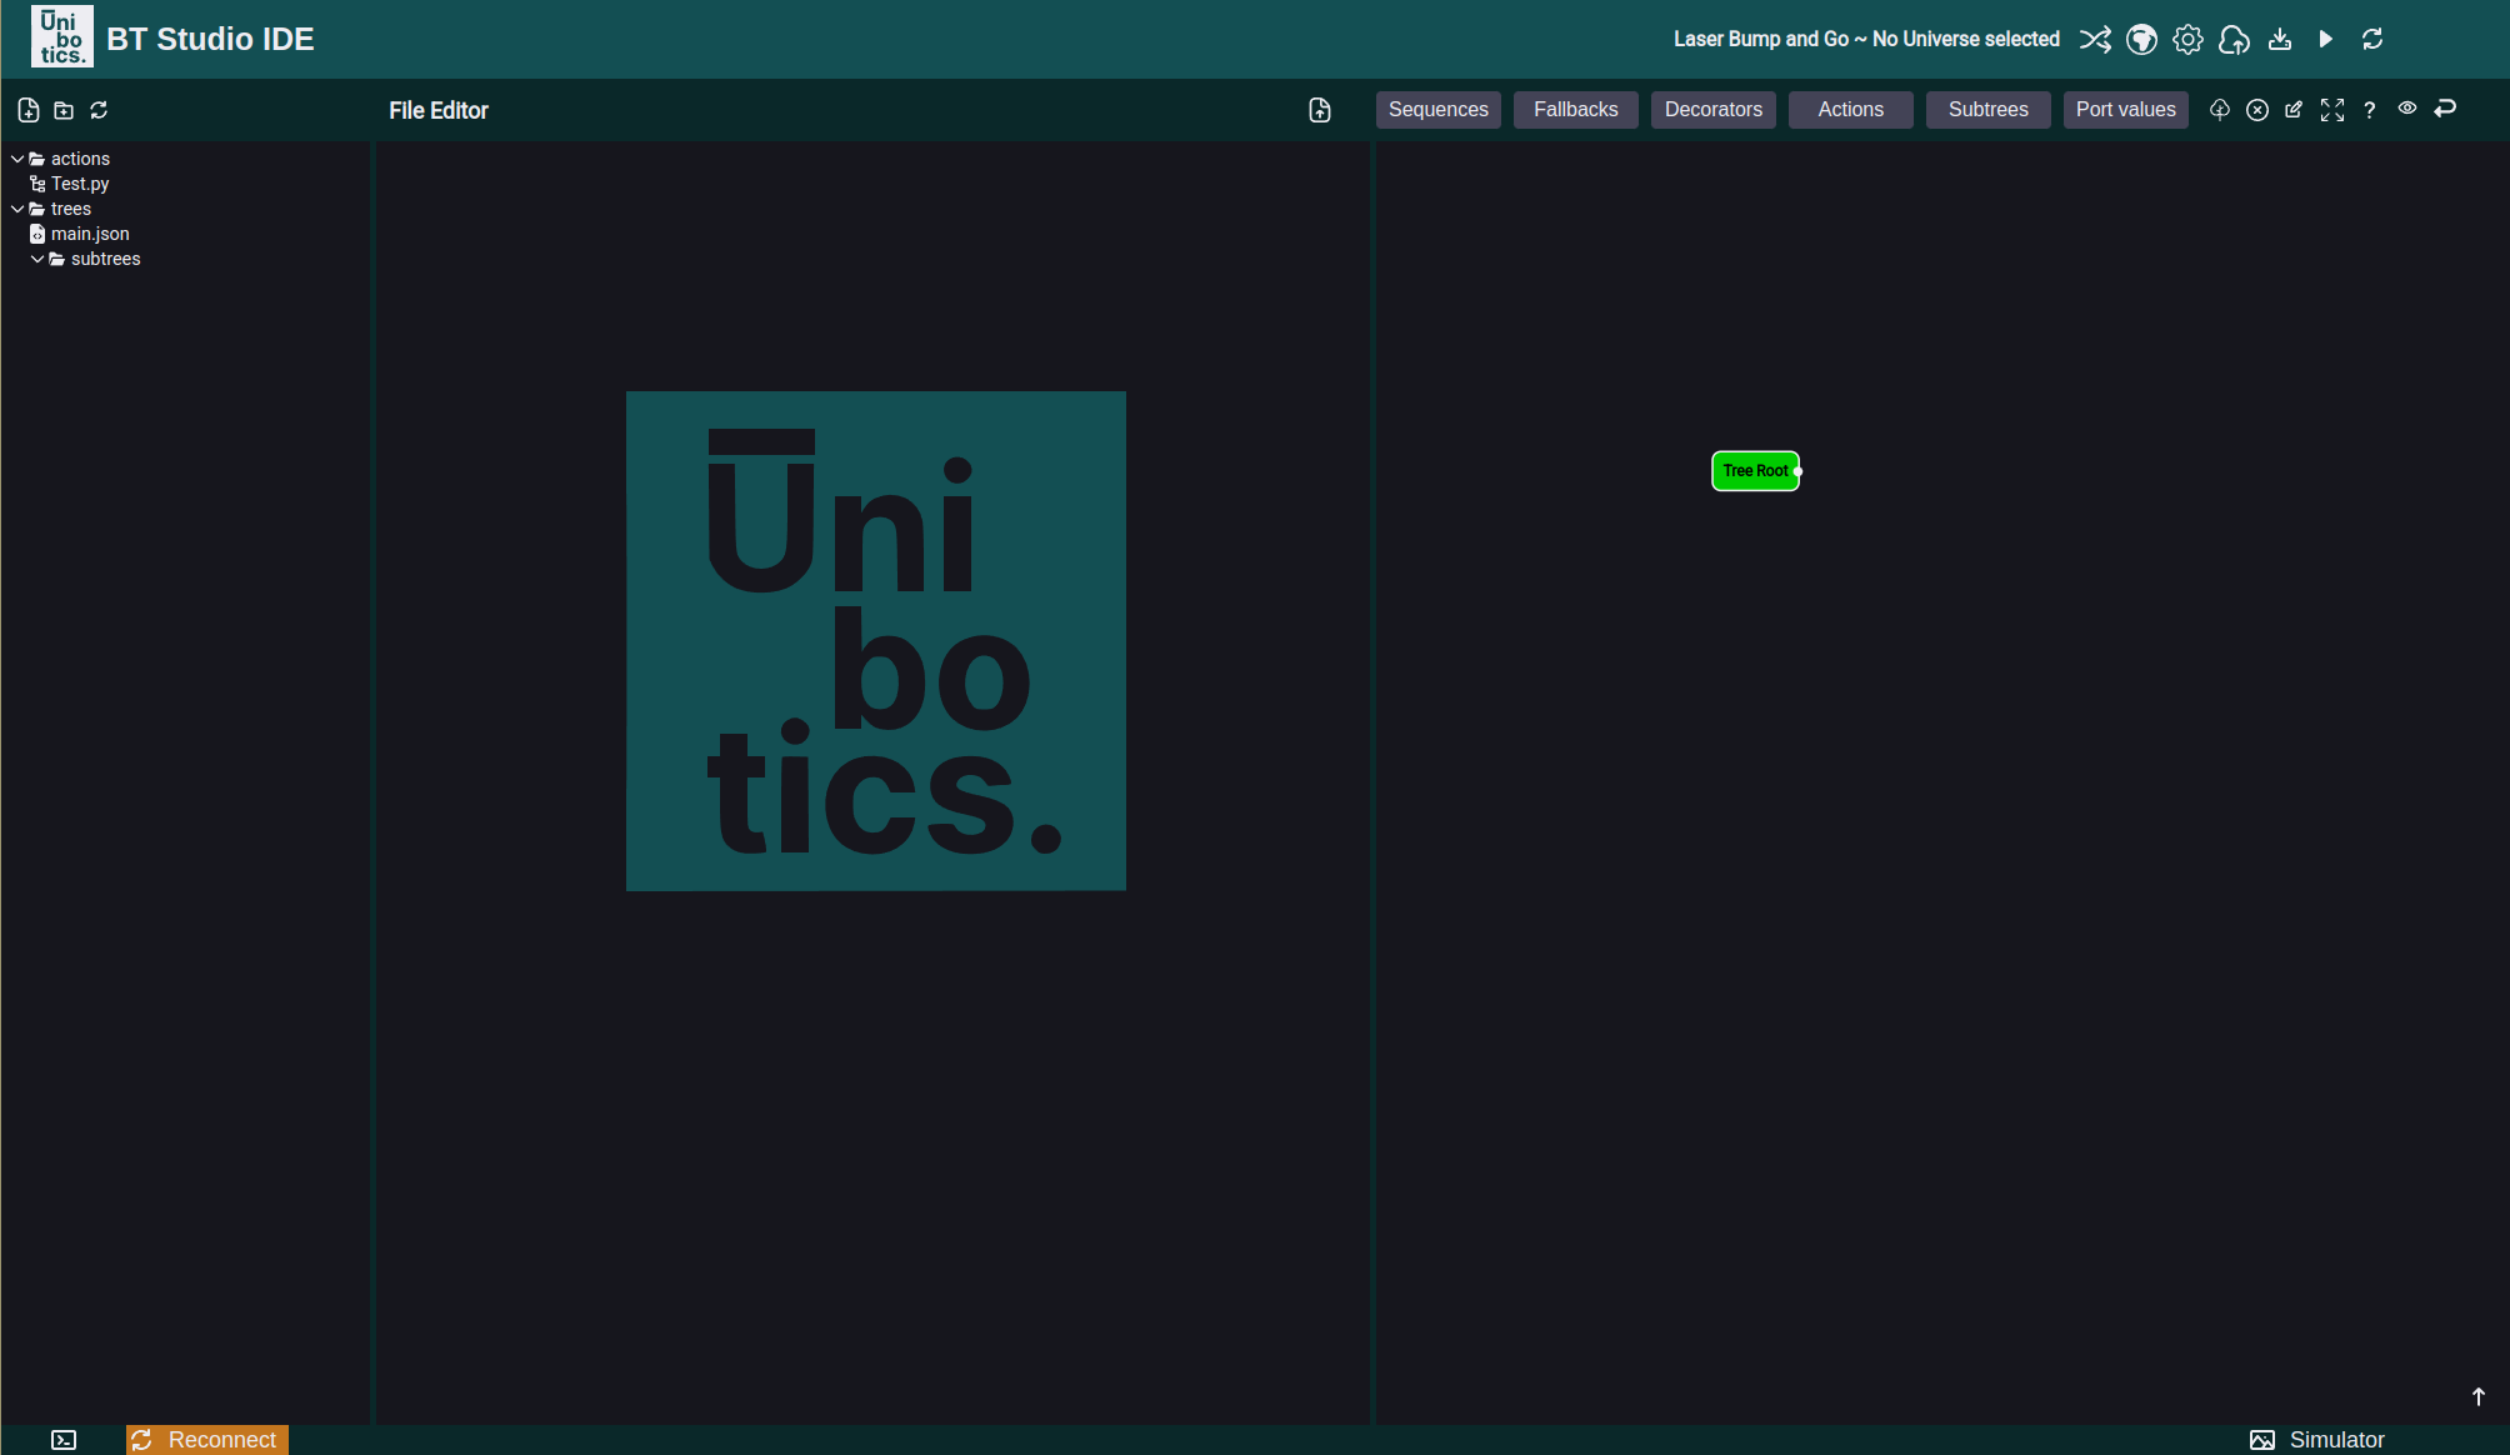
\includegraphics[width=0.9\textwidth]{figures/bt-avances/bt-unib.png}
    \caption{Apariencia de un proyecto nuevo de BT Studio en Unibotics}
    \label{fig:bt-unib}
\end{figure}

\subsection{Listado de componentes de React}

Esta sección no es una mejora, pero sirve de introducción para las que se introducirán posteriormente. Los componentes de React principales de BT Studio son:

\begin{itemize}
    \item \textbf{ErrorModal}: contiene el modal para los \textit{popups}.
    \item \textbf{FileBrowser}: contiene todo el navegador de ficheros.
    \item \textbf{FileEditor}: contiene todo el editor de ficheros Monaco.
    \item \textbf{HeaderMenu}: contiene la cabecera de BT Studio y los siguientes componentes:
    \begin{itemize}
        \item \textbf{UniverseModal}: contiene el modal para lo gestión y creación de universos.
        \item \textbf{ProjectModal}: contiene el modal para lo gestión y creación de proyectos.
    \end{itemize}
    \item \textbf{SettingsModal}: contiene el modal para las configuraciones.
    \item \textbf{StatusBar}: contiene la barra de estado.
    \item \textbf{MainTreeEditorContainer}: contiene los siguientes componentes:
    \begin{itemize}
        \item \textbf{DiagramEditor}: contiene el editor de árboles de comportamiento.
        \item \textbf{NodeMenu}: contiene los modales y acciones para el editor de árboles de comportamiento.
        \item \textbf{DiagramVisualizer}: contiene el monitor de árboles de comportamiento.
    \end{itemize}
    \item \textbf{VncViewer}: contiene el visor VNC del simulador.
    \item \textbf{TerminalViewer}: contiene el visor VNC del simulador.
\end{itemize}

\subsection{Mejora del CSS}

Esta mejora no se refleja directamente para el usuario, pero ha sido fundamental a la hora de implementar una interfaz coherente y permitir el uso de múltiples aspectos, modo claro y oscuro. La mejora ha tenido como objetivos los siguientes:

\begin{itemize}
    \item Uso de variables en el CSS para controlar los colores de los componentes.
    \item Definición de esas variables en un solo fichero, junto con los temas.
    \item Estandarización del tamaño de \textit{padding} y bordes de los componentes.
    \item Reimplementación de componentes definidos usando valores absolutos como \textit{Flexbox}.
\end{itemize}

Los dos primeros puntos han estado basados en la introducción de las variables de CSS en el código existente. Estas han sido usadas porque tienen un ámbito global y permiten que al cambiar su contenido, todas las instancias que la usan son actualizadas con este. El siguiente \textit{snippet} de código \ref{cod:css} pertenece a una versión simplificada de su uso en BT Studio.

Por último, los componentes React que usaban valores absolutos para su correcta colocación han sido reemplazados con componentes que usan el diseño \textit{Flexbox}, que permite alinear los componentes hijos en diferentes puntos usando las propiedades \textit{flex-direction}, \textit{flex-wrap}, \textit{flex-flow}, \textit{justify-content}, \textit{align-items}, \textit{align-content}. Esto consigue que los componentes se muestren de forma correcta en diferentes tamaños de pantalla.

\lstinputlisting[
    float,
    floatplacement=!htp,
    language=css,
    label=cod:css,
    caption=Ejemplo del uso de variables de CSS en BT Studio
]{code/App.css}

\subsection{Mejora de la interfaz}

La interfaz del web IDE ha tenido que ser actualizada para estar más a la última en temas de diseño y para encajar los nuevos componentes como los visores para la ejecución dockerizada que se explicarán más adelante en su propia sección.

La nueva interfaz gráfica consta de las siguientes partes que se muestran en la Figura \ref{fig:bt-int}:

\begin{itemize}
    \item Encabezado: tiene los botones para mostrar los modales de proyectos, universos y configuración, el guardado, la descarga del proyecto y el control de la ejecución. 
    \item Navegador de ficheros: permite abrir, crear y borrar ficheros y directorios. Con más detalle en su propia sección.
    \item Editor de ficheros: permite editar los ficheros y acciones del proyecto. Con más detalle en su propia sección.
    \item Barra de estado: permite controlar y ver el estado de la conexión con el entorno de ejecución dockerizada. Con más detalle en su propia sección.
    \item Editor de árboles de comportamiento: permite editar de manera visual los árboles de comportamiento. Con más detalle en su propia sección.
\end{itemize}

\begin{figure}[H]
    \centering
    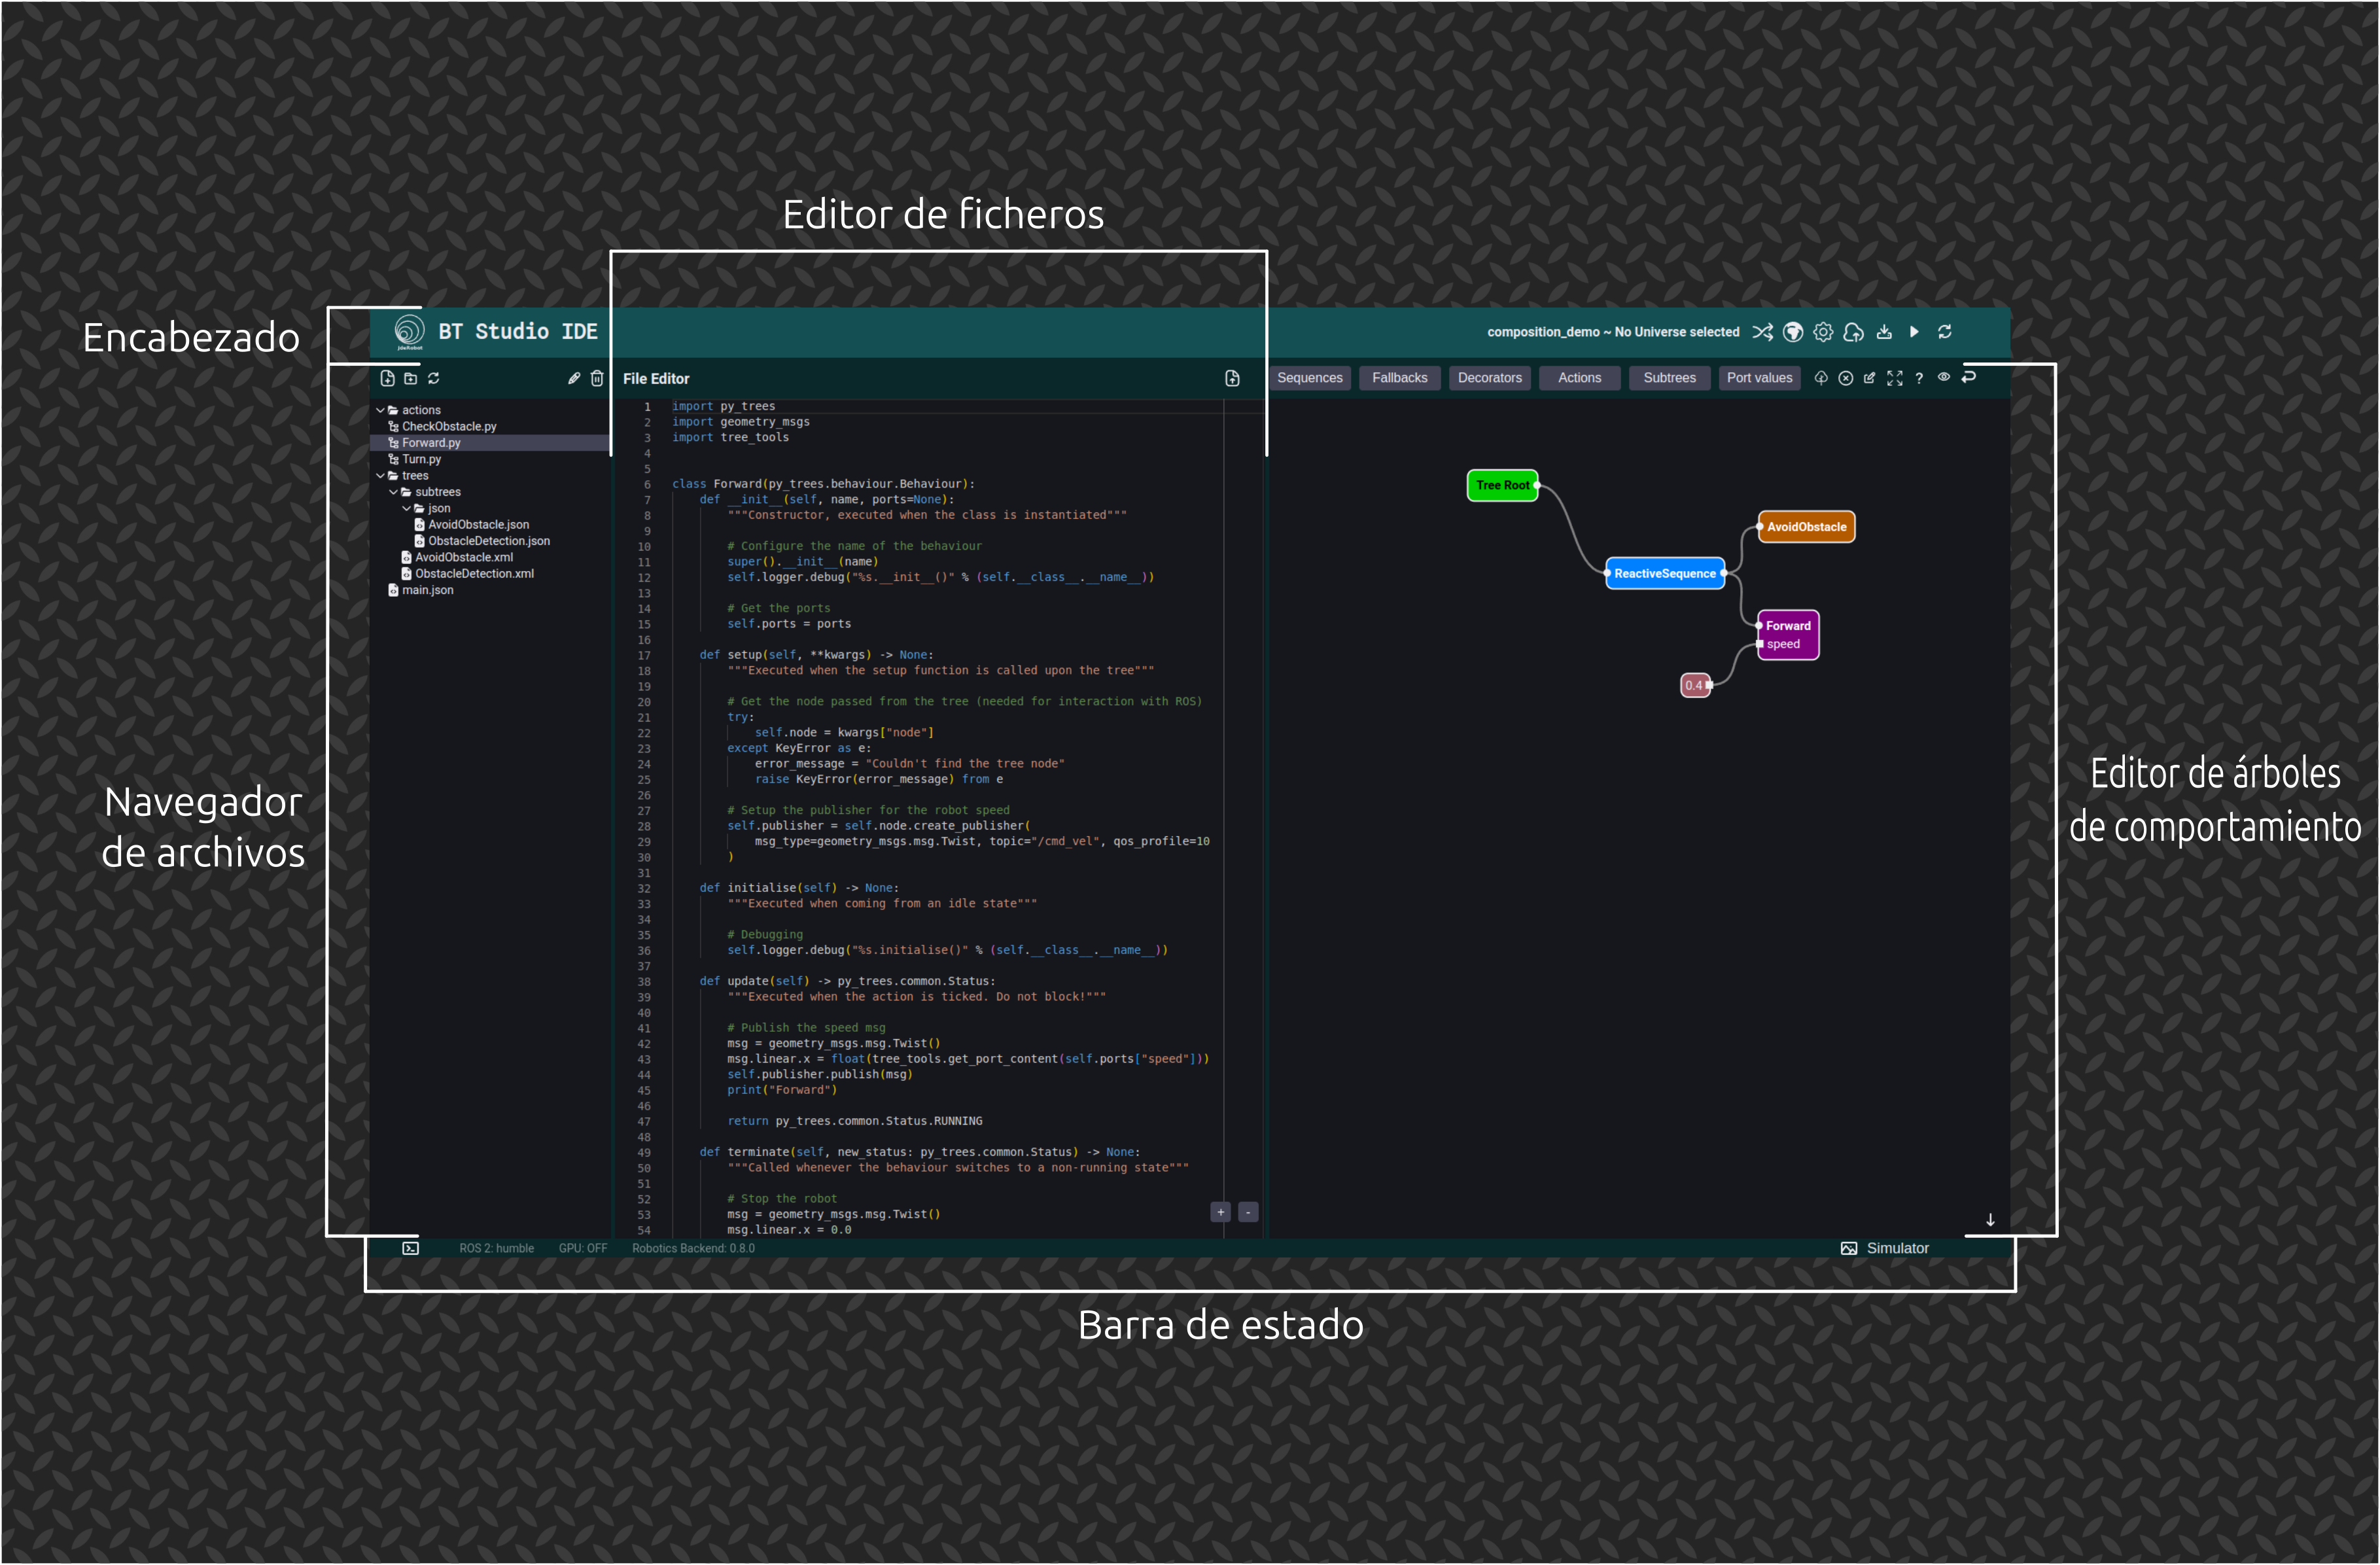
\includegraphics[width=\textwidth]{figures/bt-avances/bt-tetxo.png}
    \caption{Nueva interfaz gráfica de BT Studio sin ejecución}
    \label{fig:bt-int}
\end{figure}

Y cuando se está ejecutando la aplicación robótica en el entorno dockerizado aparecen los 2 visores que modifican la interfaz hasta parecerse a:

\begin{figure}[H]
    \centering
    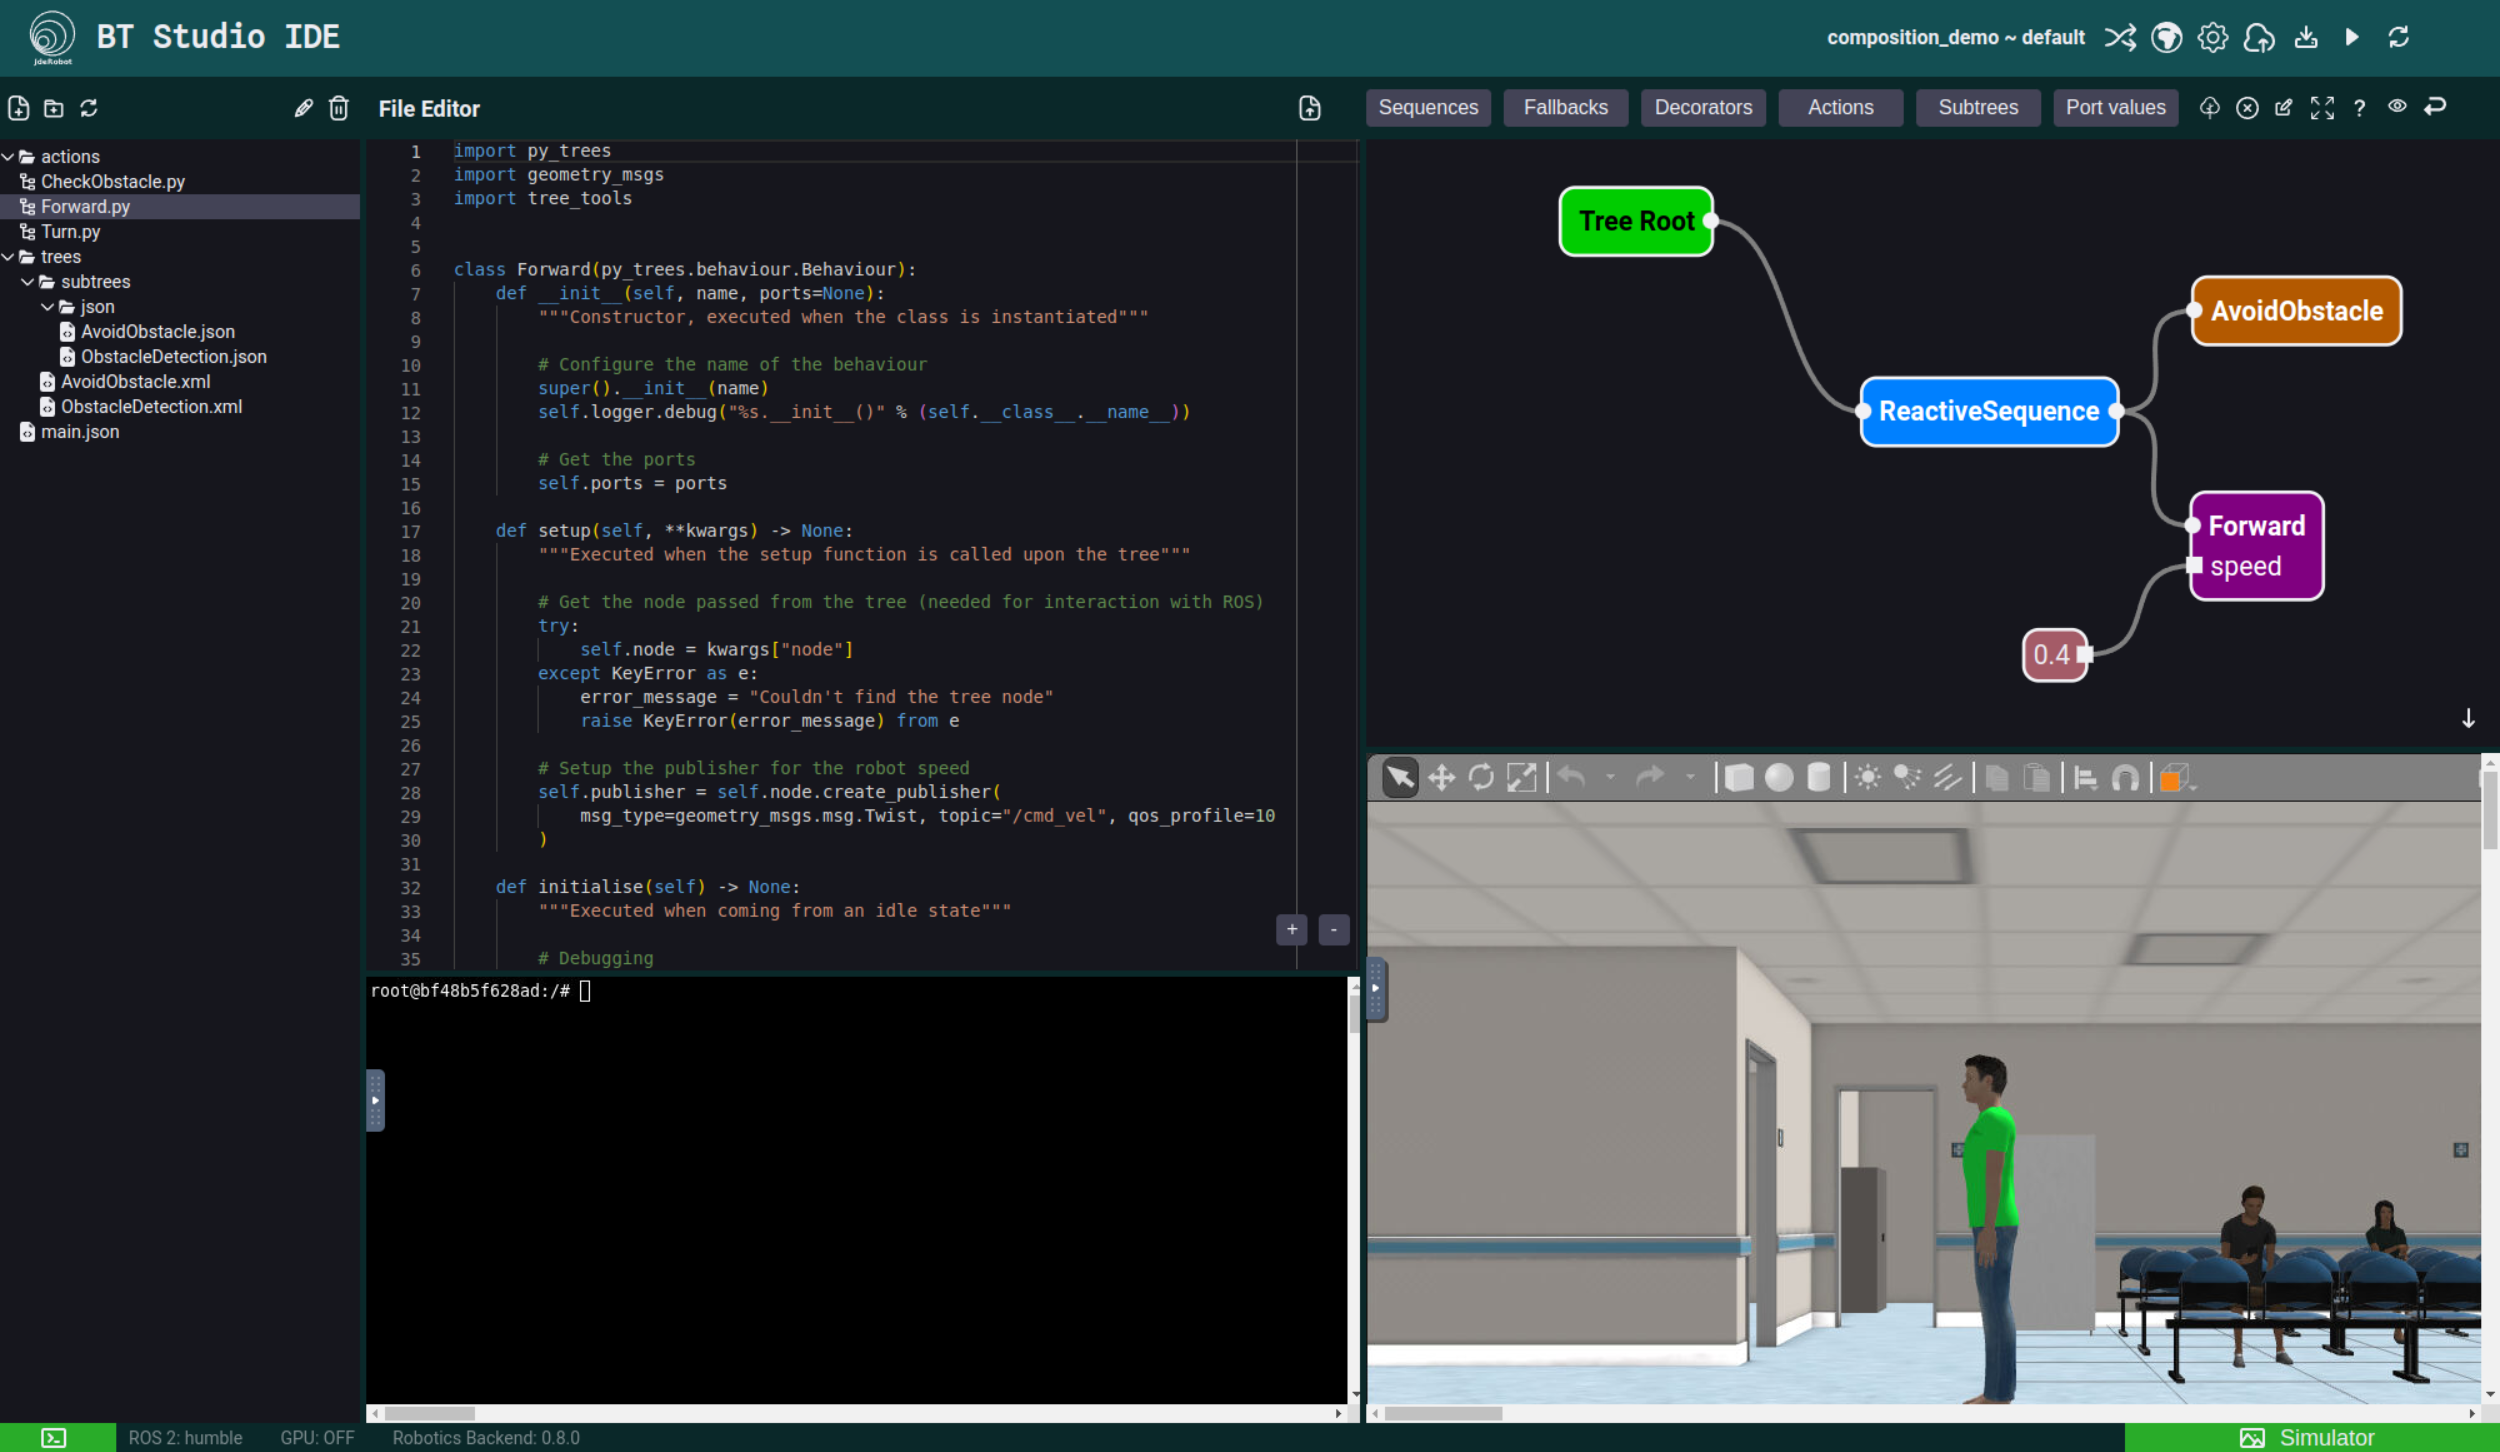
\includegraphics[width=\textwidth]{figures/bt-avances/bt-new-exec.png}
    \caption{Nueva interfaz gráfica de BT Studio en ejecución}
    \label{fig:bt-int-exec}
\end{figure}

A todos estos cambios, hay que sumarle también la posibilidad de cambiar el tema del web IDE a modo claro, que no estaba disponible en el antiguo BT Studio.

\subsection{Mejora del editor de árboles de comportamiento}\label{sec:bt-tree}

El editor de árboles de ejecución no ha quedado fuera de mejoras. Estas se pueden dividir en dos tipos: visuales y funcionales.

Las mejoras visuales corresponden a las realizadas con el fin de mejorar la apariencia del editor. Estas han sido las siguientes:

\begin{itemize}
    \item Cambio del color del fondo del editor para asemejarse al fondo del editor de ficheros y el navegador.
    \item Redondeo de los nodos del editor.
    \item Cambio del color del borde de las acciones para asemejarse al color de las letras.
    \item Cambio de los colores de los desplegables con los posibles nodos para asemejarse al resto del web IDE.
\end{itemize}

En cuanto a las mejoras funcionales, las siguientes son las que añaden algún tipo de funcionalidad nueva al editor. 

La primera y más básica de todas ellas es la prohibición de enlaces sueltos en el editor visual. Esto soluciona los problemas que se producían cuando se intentaba ejecutar una aplicación con un enlace que parecía estar conectado, pero no era el caso. Esto proporciona al usuario la confianza en que el árbol de comportamiento es tal y como se muestra para el usuario.

La segunda consiste en la adición de nuevos botones y el remplazo de otros existentes. En el primer caso, se han añadido tres nuevos botones que dan las siguientes funcionalidades: hacer zoom para centrar el árbol de comportamiento, ir a la documentación y cambiar entre el editor y el monitor de ejecución. En el otro caso, se han reemplazado los botones para añadir entradas y salidas a las acciones por uno para abrir el editor de acciones y etiquetas.

La tercera es la adición de la posibilidad de modificación del orden de ejecución del árbol de comportamiento. Esto es indicado por una flecha en la esquina inferior derecha y puede ser cambiada en el modal de configuraciones.

La cuarta modificación ha afectado a la hora de añadir múltiples instancias de una misma acción el árbol de comportamiento. Anteriormente, al añadir una nueva acción en el editor, esta se creaba sin ninguna entrada o salida, aunque hubiera una copia de esa acción ya cargada y esta tuviera alguna. Esto también ocurría al modificar las entradas y salidas de una de ellas. Para solucionar esto, ahora se guarda la información sobre todas las acciones del árbol y cuando una de estas se edita, se actualizan el resto de instancias de la acción. Esto es igual cuando se añade una copia de esa acción.

La última, al ser más compleja, se divide en los dos siguientes apartados:

\subsubsection{Editor de acciones}

Como su nombre indica, la utilidad de este es editar las acciones de una forma visual y sencilla para el usuario. Gracias a la cuarta mejora explicada anteriormente, todos los cambios a una acción se actualizarán en el resto de copias de esa acción inmediatamente. La funcionalidad que provee es la siguiente:

\begin{figure}[H]
    \centering
    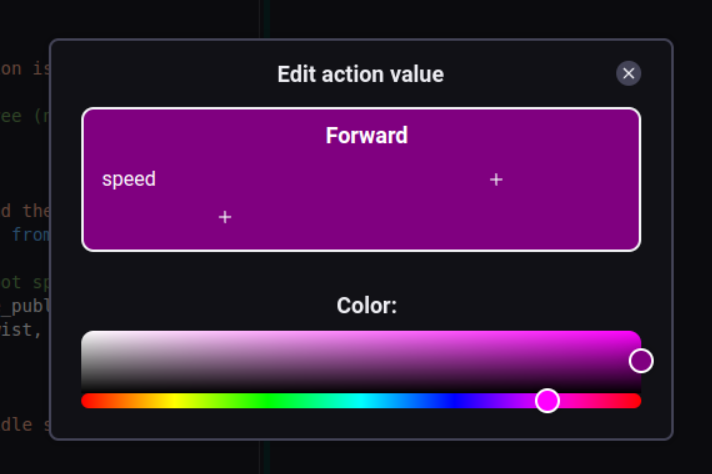
\includegraphics[width=0.5\textwidth]{figures/bt-avances/bt-edit.png}
    \caption{Editor de acciones}
    \label{fig:bt-act}
\end{figure}

\begin{itemize}
    \item Permite cambiar el color de la acción.
    \item Añadir puertos de entrada o salida siguiendo los siguientes pasos:
    \begin{enumerate}
        \item Presionar en el botón con el signo + en la columna correspondiente: izquierda para entradas y derecha para salida.
        \item Escribir el nombre del puerto.
        \item Si el nombre es válido aparecerá un botón verde para confirmar la creación del puerto, si no, solo aparecerá uno rojo para cancelarla.
        \item Presionar el botón verde para añadir el nuevo puerto.
    \end{enumerate}
    \item Borrar puertos de entrada o salida. Para esto es necesario presionar el botón rojo que aparece cuando el ratón se sitúa encima del puerto.
\end{itemize}

\subsubsection{Editor de etiquetas}

El editor de etiquetas tiene como función única permitir cambiar el contenido de la etiqueta. La única peculiaridad es que si la etiqueta se convierte a una etiqueta con acceso al \textit{blackboard}, definida en la sección \ref{sec:blackboard}, su color cambia para distinguirse de los normales en el editor.

\begin{figure}[H]
    \centering
    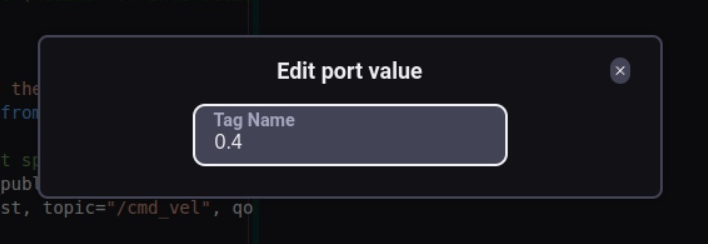
\includegraphics[width=0.6\textwidth]{figures/bt-avances/tag-edit.png}
    \caption{Editor de etiquetas}
    \label{fig:bt-tag}
\end{figure}

\subsection{Mejora del manejo de proyectos}

Se ha cambiado la forma de crear y navegar entre proyectos para que resulte más sencilla y visual al usuario. Los objetivos de esta mejora han sido los siguientes:

\begin{itemize}
    \item Substitución del \textit{popup} genérico del navegador por un modal con la lista de los proyectos creados.
    \item Reemplazar el \textit{popup} genérico del navegador por un modal para crear nuevos proyectos
    \item Permitir borrar proyectos.
\end{itemize}

Todo esto ha sido creado dentro de un solo componente, \textit{ProjectModal}, que se encuentra en el fichero \textit{frontend/src/components/header\_menu/modals/ProjectModal.tsx}. Este siempre se muestra al iniciar BT Studio, forzando al usuario a elegir un proyecto para continuar, ya que el modal no se puede cerrar si no hay un proyecto en activo.

\begin{figure}[H]
    \centering
    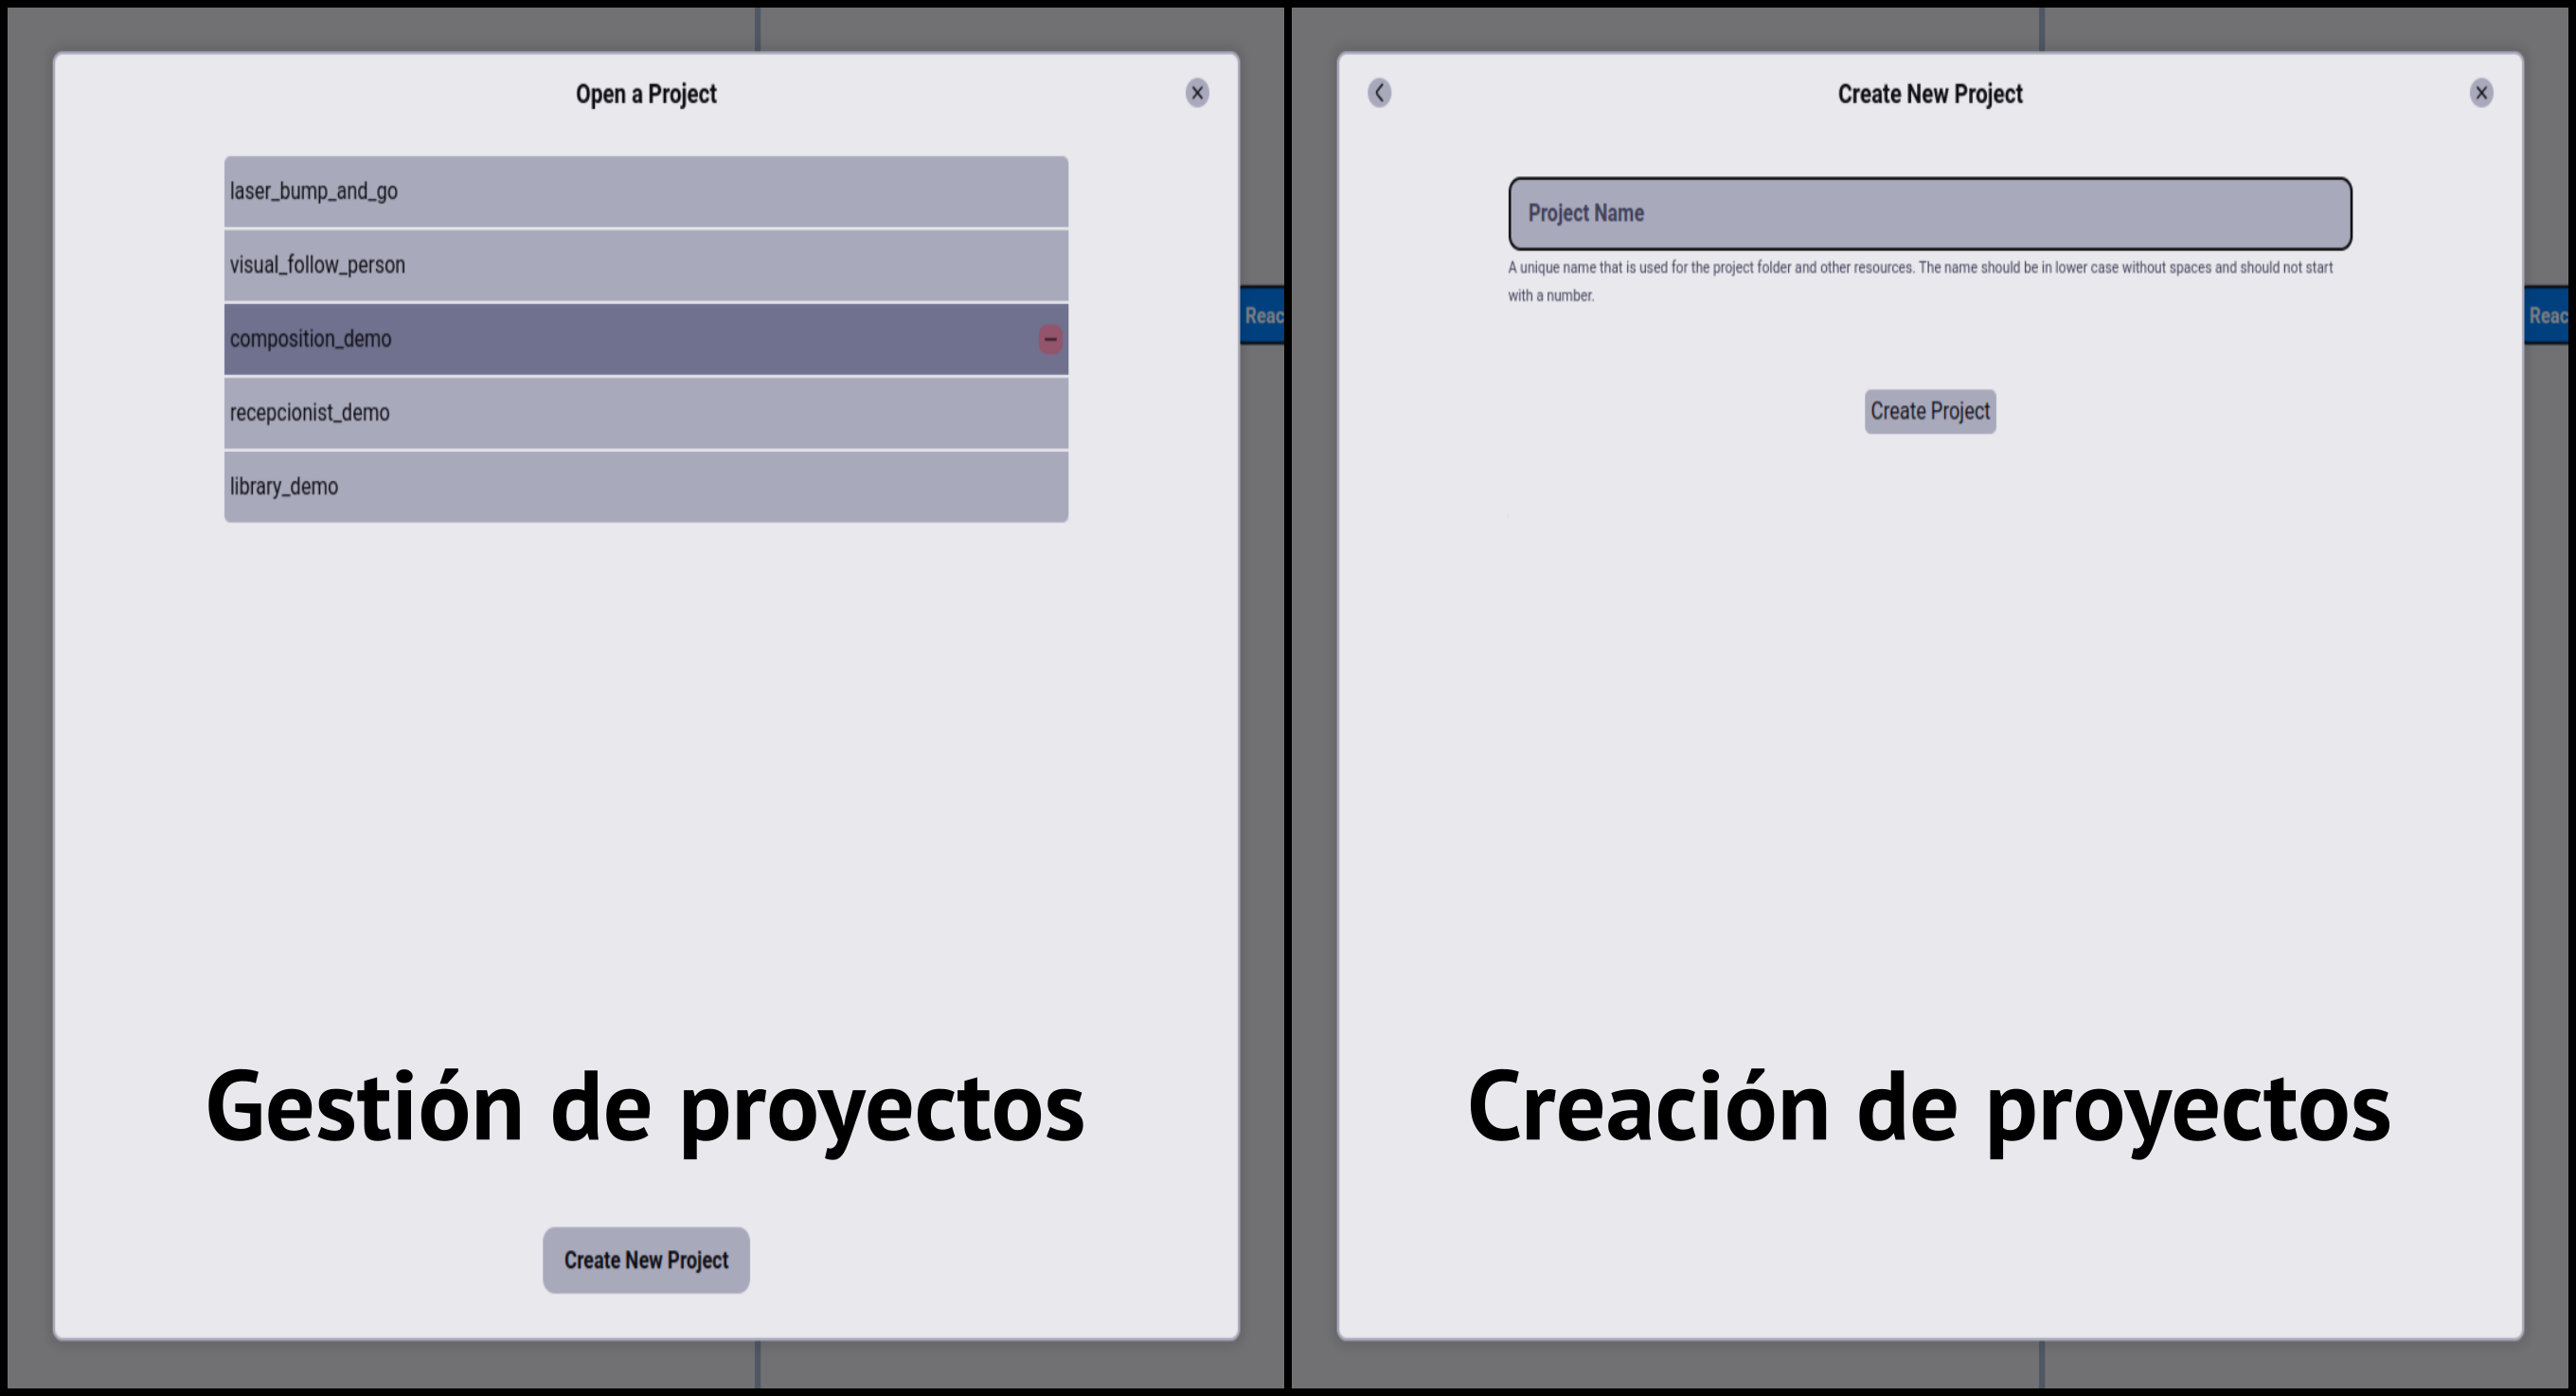
\includegraphics[width=\textwidth]{figures/bt-avances/bt-proy-2.png}
    \caption{Modales para gestión y creación de proyectos}
    \label{fig:proy-bar-rec}
\end{figure}

Al presionar encima de una de las entradas en la lista se seleccionará ese proyecto como activo y se cerrará el modal. Para poder borrar un proyecto se debe hacer clic en el botón rojo que se muestra al pasar el ratón por encima de la entrada correspondiente.

Cuando se desea crear un nuevo proyecto, después de presionar en el botón en la parte inferior del modal, este cambiará para mostrar un campo de entrada para introducir su nombre y un botón para confirmar la creación de este. 

% \begin{figure}[H]
%     \centering
%     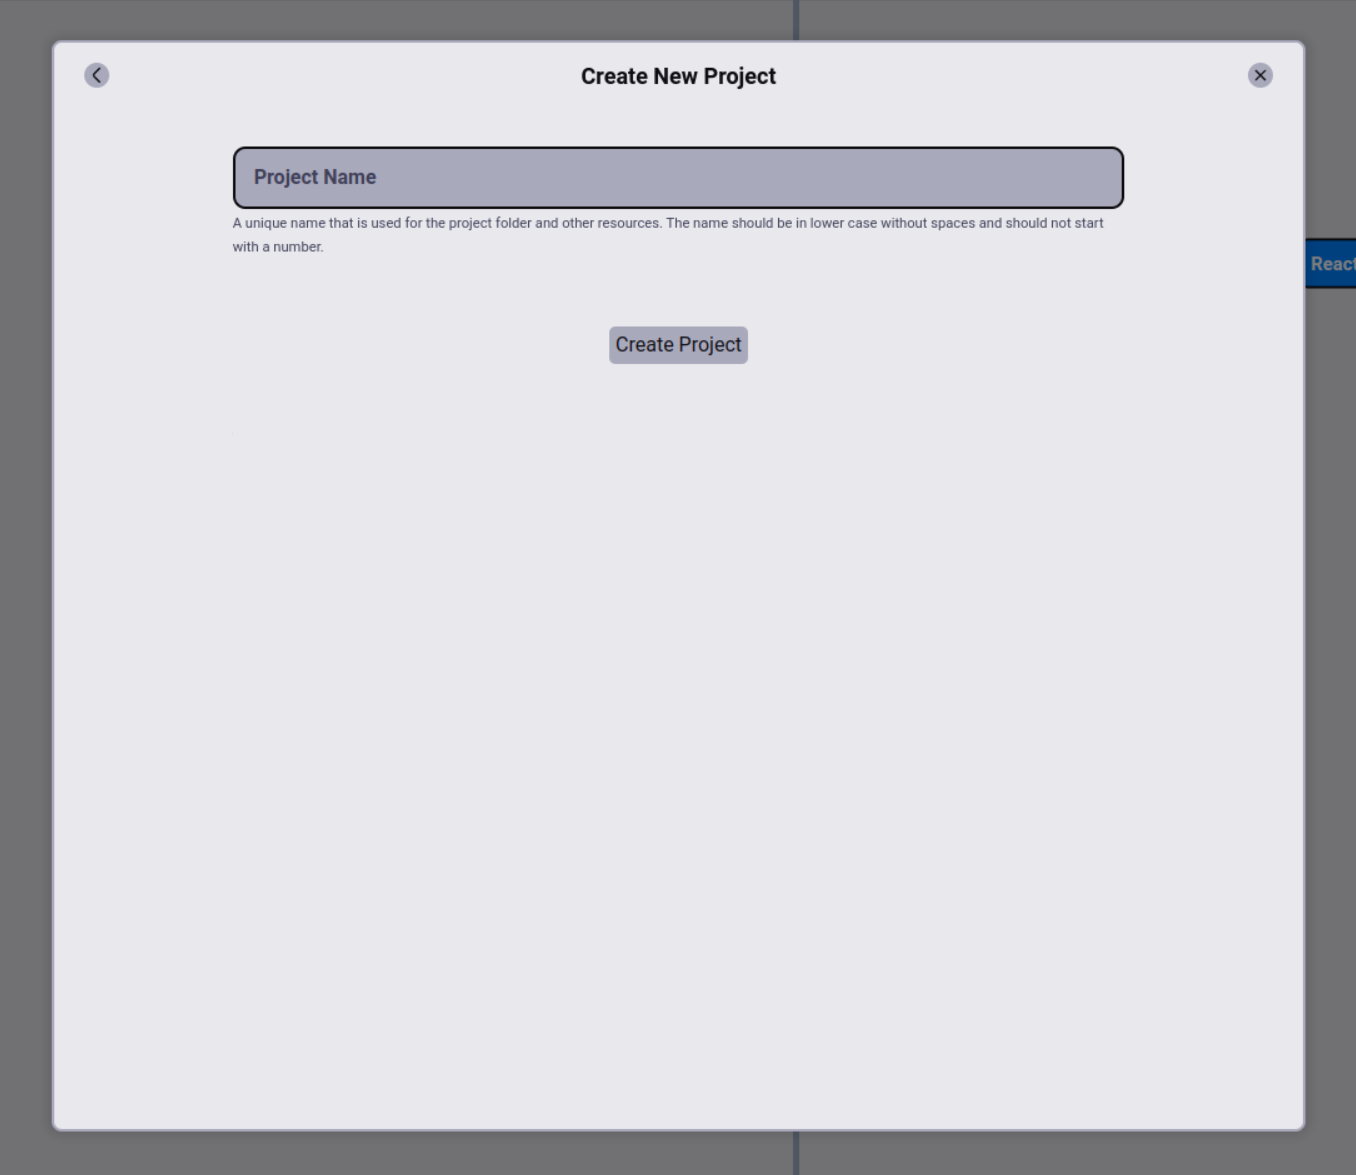
\includegraphics[width=0.5\textwidth]{figures/bt-avances/proj-create.png}
%     \caption{Apariencia del modal de proyectos}
%     \label{fig:status-bar-rec}
% \end{figure}

El modal usa los siguientes \textit{endpoints} del backend para realizar su funcionamiento:

\begin{itemize}
    \item \textbf{create\_project:} crea el nuevo proyecto.
    \item \textbf{get\_project\_list:} obtiene la lista de proyectos.
    \item \textbf{delete\_project:} borra el proyecto seleccionado.
\end{itemize} 

\subsection{Creación de la barra de estado}

La barra de estado tiene como objetivo mostrar al usuario el estado de la conexión con el entorno de ejecución dockerizado, ya sea BTDI o Robotics Backend, y permitir al usuario a forzar la conexión con este. Adicionalmente, posee un par de botones para controlar la visualización de los visores de ejecución, que se detallarán en la sección \textit{ejecución dockerizada}.

La barra de estado tiene dos estructuras diferentes dependiendo del estado de la conexión con el entorno de ejecución.

Este primero indica en naranja que no se ha podido realizar esa conexión.

\begin{figure}[H]
    \centering
    
\includegraphics[width=0.9\textwidth]{figures/bt-avances/status-bar-rec.png}
    \caption{Apariencia de la barra de estado sin conexión}
    \label{fig:status-bar-rec}
\end{figure}

Y, por otra parte, este al ya estar conectado, muestra la información sobre el entorno de ejecución.

\begin{figure}[H]
    \centering
    
\includegraphics[width=0.9\textwidth]{figures/bt-avances/status-bar.png}
    \caption{Apariencia de la barra de estado con conexión}
    \label{fig:status-bar}
\end{figure}

Para poder conseguir este funcionamiento se le deben pasar los siguientes \textit{props} al componente \textit{StatusBar} que se encuentra en el fichero \textit{frontend/src/components/status\_bar/StatusBar.tsx}:

\begin{itemize}
    \item \texttt{showSim}: indica si el visor del simulador está visible o no. 
    \item \texttt{setSimVisible}: función para cambiar la visibilidad en el visor del simulador.
    \item \texttt{showTerminal}: indica si el visor del terminal está visible o no. 
    \item \texttt{setTerminalVisible}: función para cambiar la visibilidad en el visor del terminal.
    \item \texttt{resetManager}: función para reiniciar el intento de conexión con el entorno de ejecución. Permite forzar la conexión cuando esta no es capaz de realizarse al primer intento. Cierra el intento de conexión activo del CommsManager (explicado en el capítulo \ref{cap:bt-studio}), borra el CommsManager activo, crea otra instancia y vuelve a intentar la conexión.
    \item \texttt{dockerData}: almacena la información sobre el entorno de ejecución dockerizada. 
\end{itemize}

\subsection{Mejora del editor}\label{sec:bt-monaco}

El editor de archivos ha sido reemplazado por completo, pasando de ACE \footnote{\url{https://ace.c9.io}} a Monaco \footnote{\url{https://microsoft.github.io/monaco-editor/}}. Este último es un editor creado por Microsoft y que es usado en el popular editor VS Code, pero que continúa siendo \textit{open source} bajo la licencia MIT.

\begin{figure}[H]
    \centering
    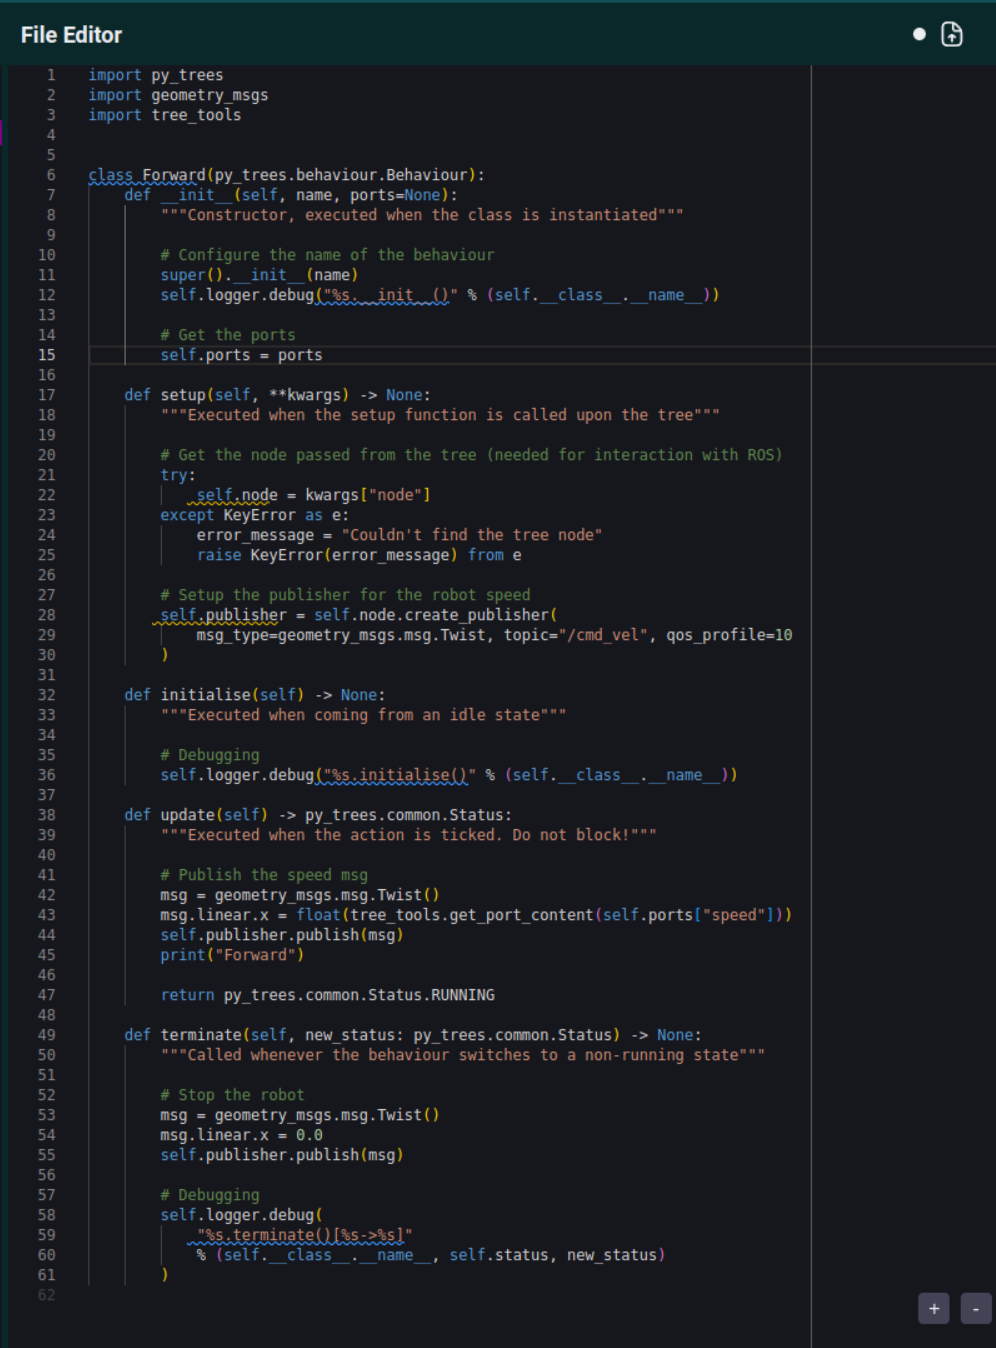
\includegraphics[width=0.6\textwidth]{figures/bt-avances/editor.png}
    \caption{Editor de archivos}
    \label{fig:bt-editor}
\end{figure}

Este nuevo editor ofrece una apariencia más moderna y varias mejoras de funcionalidad sobre ACE. Las que más interesan para BT Studio son las siguientes:

\begin{itemize}
    \item Soporte para búsqueda en el código usando \textbf{Ctrl + F}.
    \item Personalización más sencilla usando temas.
    \item Soporte para \textit{snippets} personalizados y autocompletado.
    \item Soporte para el resaltado de código para varios lenguajes de programación.
\end{itemize}

Gracias a todas estas funcionalidades se ha añadido al editor de BT Studio la capacidad de realizar las siguientes acciones siempre que se esté conectado al entorno de ejecución dockerizado gracias a la mediación del CommsManager, ya que este es capaz de intercambiar mensajes con el RAM donde se realiza el cómputo de todas las funciones que se van a detallar a continuación:

\begin{itemize}
    \item Formateo de código usando el formateador de Python. \textit{black}\footnote{\url{https://pypi.org/project/black/}}. Se activa desde el web IDE usando \textbf{Ctrl + Shift + I} y solo funciona para los ficheros de Python.
    \item Resaltado de código automático usando el \textit{linter} de Python \textit{pylint}\footnote{\url{https://pypi.org/project/pylint/}}. Solo funciona para los ficheros de Python. 
    \item Soporte para autocompletado de código usando \textit{jedi}\footnote{\url{https://pypi.org/project/jedi/}}, solo disponible para los ficheros de Python.
\end{itemize}

Todas estas funciones han sido añadidas desde este TFG en el Robotics Application Manager.

\subsection{Creación de \textit{popups}}

Para finalizar, la última mejora es la introducción de \textit{popups} para mostrar información al usuario que antes solo se encontraba en las trazas para desarrolladores. Estos han sido creados usando el mismo proceso que con las configuraciones, es decir, usando el elemento \textit{context} de React y envolviéndolo en un proveedor, \textit{ErrorProvider} que está localizado en el fichero \textit{frontend/src/components/error\_popup/ErrorModal.tsx}, y que se añade a la aplicación en el fichero \textit{frontend/src/index.js} para que esté disponible en toda la aplicación.

Con esto dicho, podemos pasar a mostrar cada uno de los tres tipos de \textit{popups}, así como su utilidad y forma de uso.

\subsubsection{\textit{Popup} de error}
\begin{itemize}
    \item Finalidad: mostrar al usuario que ha ocurrido un error. Se permite cerrar la ventana emergente sin problema.
    \item Forma de uso: usando la función \textit{error()} pasandole como parámetro el mensaje de error.
\end{itemize}
\begin{figure}[H]
    \centering
    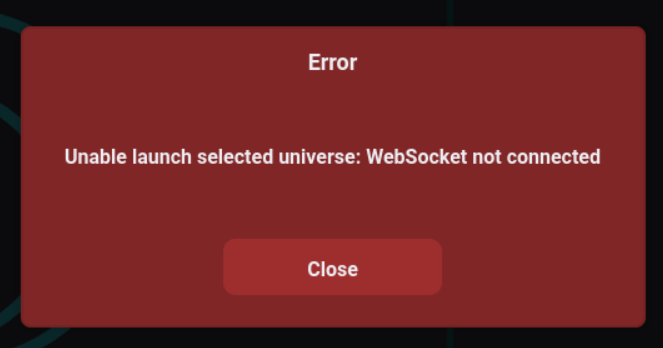
\includegraphics[width=0.55\textwidth]{figures/bt-avances/error.png}
    \caption{Popup de error}
    \label{fig:bt-err}
\end{figure}

\subsubsection{\textit{Popup} de error crítico}
\begin{itemize}
    \item Finalidad: mostrar al usuario que ha ocurrido un error y salir de la aplicación.
    \item Forma de uso: usando la función \textit{error\_critical()} pasandole como parámetro el mensaje de error.
    \item El aspecto es el mismo al de uno de error normal.
\end{itemize}

\subsubsection{\textit{Popup} de aviso}
\begin{itemize}
    \item Finalidad: mostrar al usuario que hay un aviso, normalmente porque algo no se está haciendo de forma correcta. Se permite cerrar la ventana emergente sin problema.
    \item Forma de uso: usando la función \textit{warning()} pasandole como parámetro el mensaje de error.
\end{itemize}
\begin{figure}[H]
    \centering
    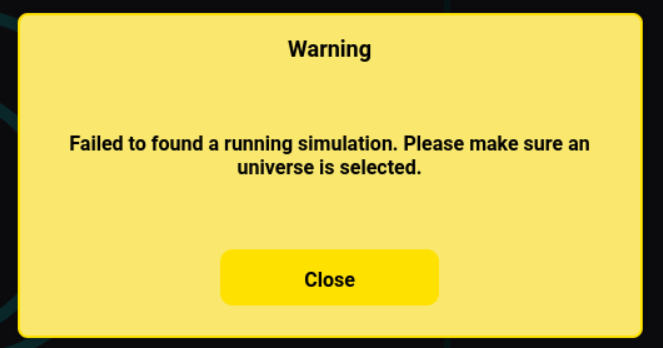
\includegraphics[width=0.55\textwidth]{figures/bt-avances/warning.png}
    \caption{Popup de aviso}
    \label{fig:bt-warn}
\end{figure}

\subsubsection{\textit{Popup} de información}
\begin{itemize}
    \item Finalidad: mostrar al usuario alguna información que no es ni un aviso ni un error. Se permite cerrar la ventana emergente sin problema.
    \item Forma de uso: usando la función \textit{info()} pasandole como parámetro el mensaje de error.
\end{itemize}
\begin{figure}[H]
    \centering
    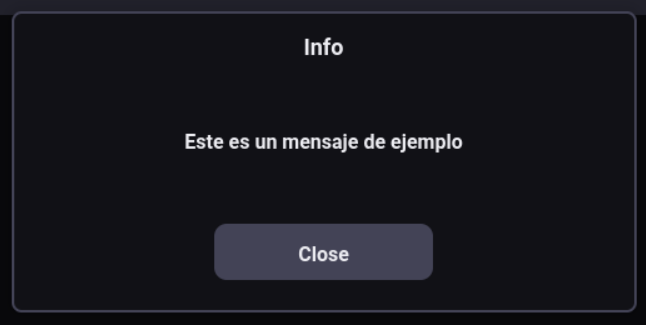
\includegraphics[width=0.55\textwidth]{figures/bt-avances/info.png}
    \caption{Popup de información}
    \label{fig:bt-info}
\end{figure}

\section{Navegador de archivos}

El navegador de archivos ha sido re-implementado completamente para adecuarse a un uso más generalizado y con más funcionalidad, ya que el editor antiguo solo podía crear acciones vacías y solo mostraba y dejaba eliminar estas acciones. Estos cambios permiten editar cualquiera de los ficheros de un proyecto, menos aquellos que se encuentran dentro del directorio \textit{trees}, debido a que cambios en estos pueden causar que se rompa el editor de árboles de comportamiento.

\begin{figure}[H]
    \centering
    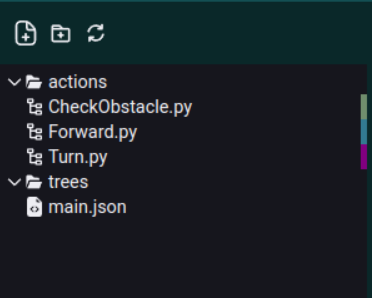
\includegraphics[width=0.3\textwidth]{figures/bt-avances/nav.png}
    \caption{Apariencia del navegador de archivos sin ninguno abierto}
    \label{fig:nav-close}
\end{figure}

El nuevo componente permite las siguientes funciones:

\begin{itemize}
    \item Mostrar todo el contenido del directorio \textit{code} del proyecto.
    \item Crear, renombrar y borrar ficheros.
    \item Crear, renombrar y borrar directorios.
    \item Crear acciones usando plantillas.
    \item Descargar ficheros o directorios.
    \item Subir ficheros al proyecto.
    \item Mostrar el color de la acción correspondiente del editor de árboles de comportamiento.
\end{itemize}

Para conseguir lo primero se ha implementado un navegador de ficheros que puede colapsar los directorios y que tabula los ficheros dentro de estos para poder visualizarlo de forma clara.

% \begin{figure}[H]
%     \centering
%     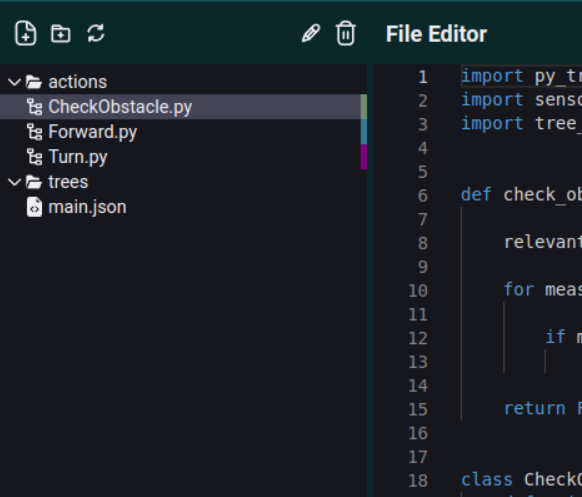
\includegraphics[width=0.4\textwidth]{figures/bt-avances/nav-open.png}
%     \caption{Apariencia del navegador de archivos con un fichero abierto}
%     \label{fig:nav-open}
% \end{figure}

En cuanto a los siguientes puntos, la mayoría de estos puede ser activados de dos maneras distintas: usando los botones disponibles en la parte superior del navegador o con el que aparece al mantener el ratón encima de esa entrada. Al hacerlo de esta última forma aparecerá un menú de contexto que tiene diferentes opciones dependiendo del fichero o directorio donde se ha activado.

\begin{figure}[H]
    \centering
    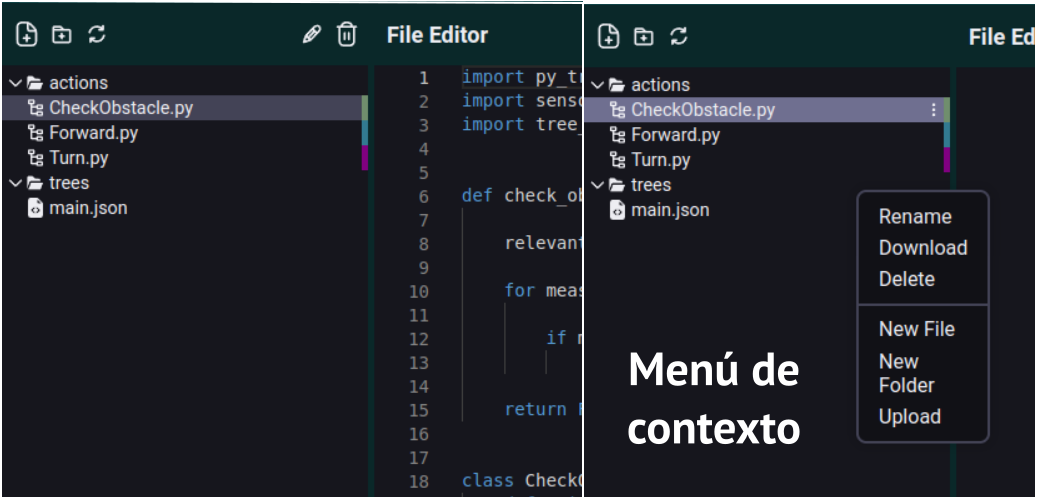
\includegraphics[width=\textwidth]{figures/bt-avances/bt-nav-2.png}
    \caption{Apariencia del menú de contexto del navegador de archivos}
    \label{fig:nav-menu}
\end{figure}

Todas las opciones disponibles abrirán un nuevo modal donde se podrán realizar la acción correspondiente, y si esta conlleva la creación o la subida de ficheros o directorios, se tendrá en cuenta la última entrada seleccionada en el modal para ser el lugar donde se lleve a cabo la acción. Estos modales son:

\subsubsection{Creación de ficheros y acciones}

Permite crear un fichero con el nombre escrito por el usuario. Solo si ese nombre es válido, es decir, no existe ya uno en ese lugar, se permite su creación.

\begin{figure}[H]
    \centering
    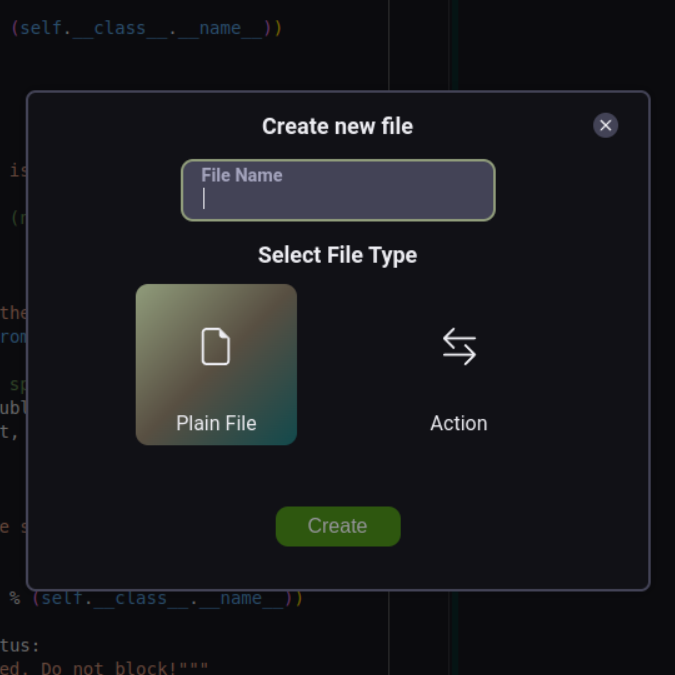
\includegraphics[width=0.5\textwidth]{figures/bt-avances/new-file.png}
    \caption{Modal de creación de ficheros}
    \label{fig:bt-file-new}
\end{figure}

Si se quiere crear una acción, es decir, un fichero de Python en un directorio especial, se debe primero seleccionar la opción de \textit{Acción} y luego seleccionar el tipo de plantilla que se desea: vacía, acción normal o acción con puertos. Como la acción siempre es un archivo de Python, se considera inválido su nombre, si además de lo definido anteriormente, posee algún punto o acaba en \textbf{.py}.

\begin{figure}[H]
    \centering
    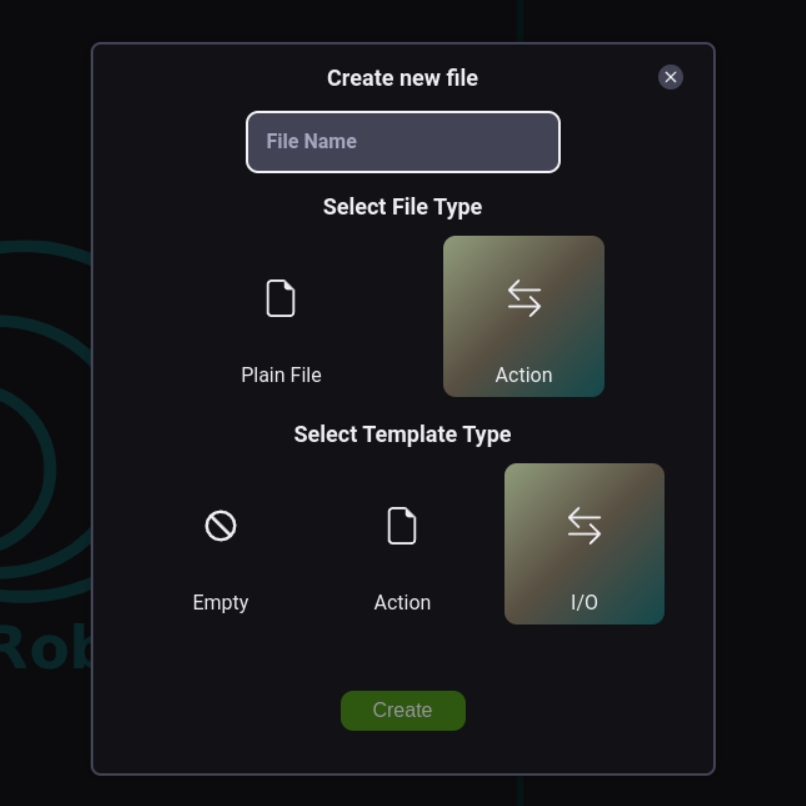
\includegraphics[width=0.5\textwidth]{figures/bt-avances/new-action.png}
    \caption{Modal de creación de acciones}
    \label{fig:bt-action-new}
\end{figure}

\subsubsection{Creación de directorios}

Permite crear un directorio con el nombre escrito por el usuario. Solo si ese nombre es válido, es decir, no existe ya en ese lugar, se permite su creación.

\begin{figure}[H]
    \centering
    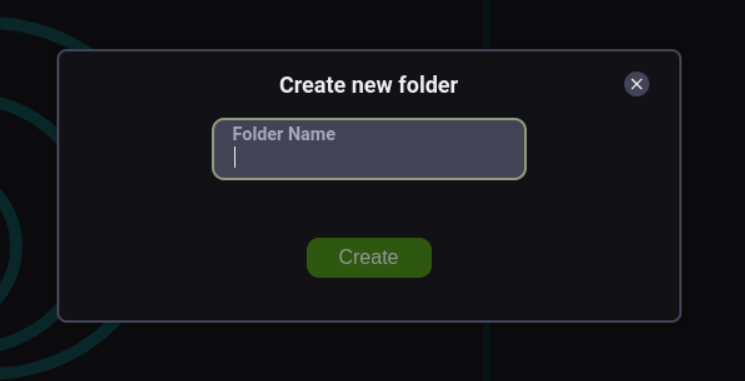
\includegraphics[width=0.5\textwidth]{figures/bt-avances/bt-folder-new.png}
    \caption{Modal de creación de directorios}
    \label{fig:bt-dir-new}
\end{figure}

\subsubsection{Renombrar ficheros y directorios}

Permite renombrar un fichero o directorio con el nombre escrito por el usuario. Solo si ese nombre es válido, es decir, no existe ya en ese lugar, se permite renombrarlo.

\begin{figure}[H]
    \centering
    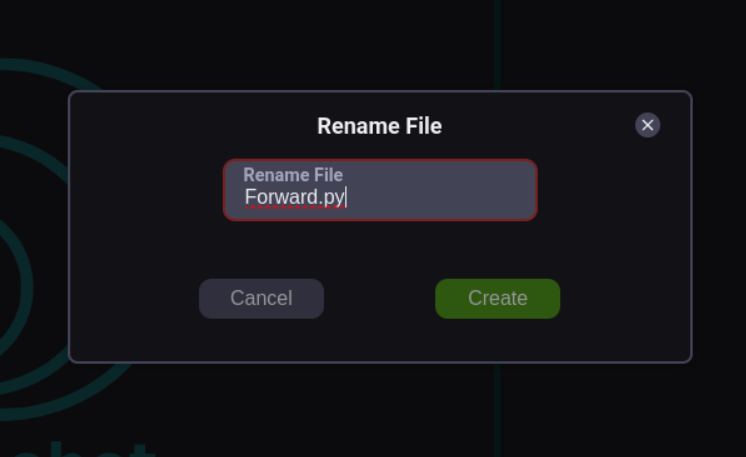
\includegraphics[width=0.5\textwidth]{figures/bt-avances/bt-rename.png}
    \caption{Modal de renombrar de directorios o ficheros}
    \label{fig:bt-rename}
\end{figure}

\subsubsection{Eliminar ficheros y directorios}

Muestra una ventana emergente para confirmar la eliminación del fichero o directorio seleccionado

\begin{figure}[H]
    \centering
    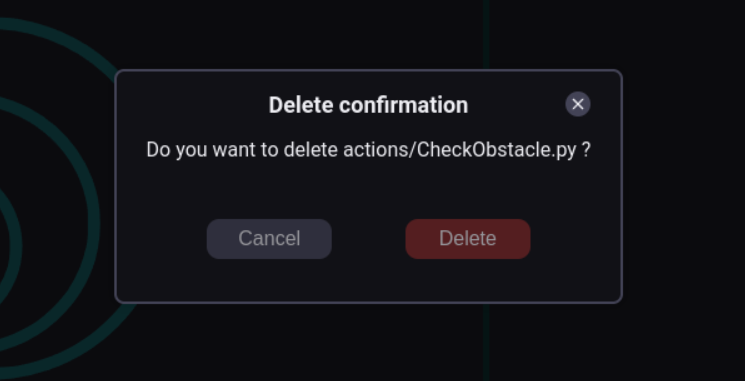
\includegraphics[width=0.5\textwidth]{figures/bt-avances/bt-del.png}
    \caption{Modal de eliminar directorios o ficheros}
    \label{fig:bt-delete}
\end{figure}

\subsubsection{Subir ficheros}

Permite subir ficheros desde el ordenador del usuario al proyecto

\begin{figure}[H]
    \centering
    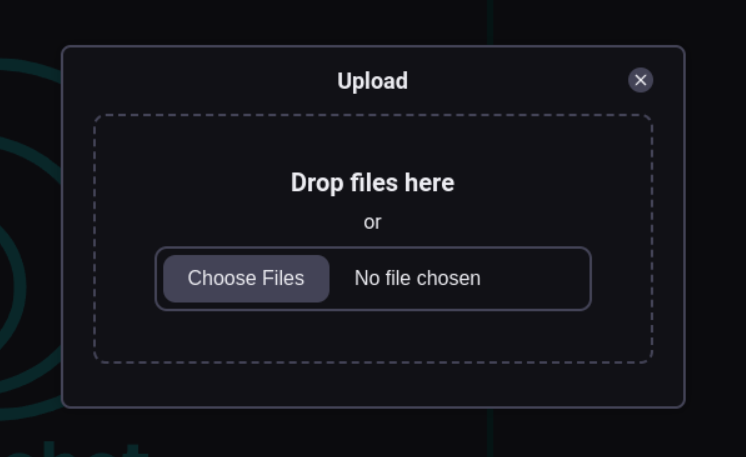
\includegraphics[width=0.5\textwidth]{figures/bt-avances/bt-upload.png}
    \caption{Modal para subir ficheros}
    \label{fig:bt-upload}
\end{figure}

\section{Universos}

La adición de universos a BT Studio ha sido clave en la mejora de la experiencia del usuario a la hora de ejecutar las aplicaciones robóticas en el entorno dockerizado. La forma de cómo se lanza cada universo en el entorno dockerizado será explicado en su propia sección, \textit{ejecución dockerizada}. Antes de explicar esto en más detalle, se debe definir qué es un universo.

Se considera un universo a la combinación de un mundo y un robot, y en este caso en formatos que utiliza el simulador Gazebo. Estos universos deben tener además un punto de entrada para ser lanzados, y como se usa ROS2, este será un \textit{launcher}.

Con todo esto ya definido, el usuario tiene acceso a dos tipos de universos: los predefinidos en el Robotics Backend y los suyos personalizados. Para poder controlar y navegar entre los distintos universos se crea un nuevo modal que permite crear, eliminar y cambiar estos.

\begin{figure}[H]
    \centering
    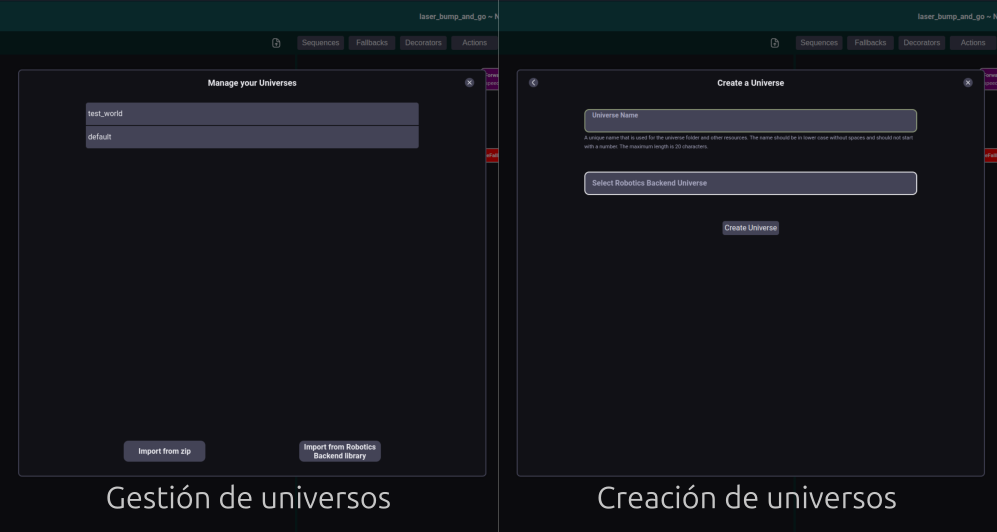
\includegraphics[width=\textwidth]{figures/bt-avances/bt-univ.png}
    \caption{Modales para gestión y creación de universos}
    \label{fig:bt-univ}
\end{figure}

\subsection{Universos personalizados}

Para añadir un universo propio del usuario, este debe primero comprimir todos los ficheros que lo componen en un archivo ZIP y llamarlo con el nombre que quiere que aparezca en BT Studio. Por último, se debe presionar en el botón correspondiente en la esquina inferior izquierdo y subir el archivo del universo.

Estos universos solo tendrán soporte para la versión del simulador Gazebo, Harmonic.

\subsection{Universos del Robotics Backend}

Para poder utilizar estos universos en BT Studio se ha tenido que realizar un trabajo previo en Robotics Infrastructure (RI), Robotics Academy (RA) y en la propia forma de lanzar BT Studio. Esta última parte ya se ha explicado anteriormente en el apartado \ref{sec:uso-bt}.

El trabajo que se ha realizado en RI y en RA ha consistido primero en migrar las bases de datos de este último de SQLite a PostgreSQL con el objetivo de usar las mismas bases de datos que Unibotics, y posteriormente separar los universos en su propia base de datos y ubicarla en el repositorio de Robotics Infrastructure. Esto permitía usar la misma base de datos con los universos en Robotics Academy y en Unibotics, mejorando la experiencia del desarrollador y facilitando el mantenimiento.

El problema que surgía con estos cambios era que al usar PostgreSQL se necesita lanzar su propio servicio en un puerto del usuario y esto hacía que no fuera posible contenerlo todo dentro de un mismo contenedor docker. Para solucionarlo, se crea un nuevo contenedor basado en la imagen de PostgreSQL disponible en \textit{dockerhub} y gracias a la herramienta \textit{docker-compose} se lanzan los dos contenedores docker usando un solo fichero de configuración sin necesidad de instalar y correr PostgreSQL en local. Esto junto con la propiedad \textit{bind} de docker permite reemplazar el contenido de la base de datos con la que esté disponible en local, haciendo que el desarrollo de cambios en estas bases de datos sea sencillo para probar.

Pero con esto último volvía a aparecer otro problema, y era dónde situar la base de datos para que fuera cargada. Para esto se introdujo Robotics Infrastructure como submódulo en BT Studio y en Robotics Academy, ya que esto conseguía que la base de datos se mantuviera en un solo lugar, RI, pero se pudiera acceder a ella desde múltiples aplicaciones.

Con todo este trabajo previo ya realizado, ha hecho falta también adaptar la parte de Django de BT Studio para que entendiera y se conectará con el docker que contiene la base de datos de universos.

Ahora que BT Studio ya es capaz de acceder y mostrar las entradas de la base de datos de universos, al usuario se le muestra un campo de entrada para escribir el nombre del universo, y un desplegable para que elija entre la lista de los universos disponibles, como se muestra en la figura \ref{fig:bt-univ}.

Estos universos tienen soporte para las versiones del simulador Gazebo, Harmonic y Classic.

\section{Monitor de ejecución}\label{sec:bt-monitor}

La adición del monitor de ejecución provee al usuario de una manera visual y sencilla de observar el estado del árbol de comportamiento de la aplicación robótica. Este monitor está inspirado por el disponible en la aplicación \textit{Groot2} nombrada en la introducción y completa el objetivo restante de BT Studio, poseer de herramientas para la depuración de aplicaciones.

Este monitor se sitúa en el mismo lugar que el editor de árboles de comportamiento y se cambia de vista presionando el botón con forma de ojo que se halla presente en ambos. Para que el monitor de ejecución se haya podido crear, ha habido que trabajar en tres frentes distintos: el frontend, el backend y el entorno dockerizado.

\subsection{Backend}

En el backend ha hecho falta traducir el árbol de comportamiento a una lista con sus componentes simplificados, estando los nodos hijos contenidos como listas dentro de los padres. Esto ha sido posible gracias a la reutilización del traductor de JSON a XML ya existente, y que está explicado en más detalle en el TFG \cite{TFG_BT_Studio}, y un par de cambios. Gracias a este esqueleto generado se pueden situar los estados en las acciones adecuadas en el diagrama del monitor.

\subsection{Frontend}

Este recibe información de dos sitios para crear el diagrama final: del backend recibe el esqueleto del árbol y del entorno dockerizado recibe el estado actual de los nodos en todo momento. Todo esto, junto con el árbol de comportamiento original, permite mostrar sus estados de forma correcta en tiempo real.

Como el monitor de ejecución no debe permitir la edición del árbol de comportamiento, el diagrama mostrado no puede ser editado de ninguna manera, es decir, bloquea todo tipo de movimiento de nodos, su eliminación o su edición con los modales explicados en el apartado \ref{sec:bt-tree}.

\begin{figure}[H]
    \centering
    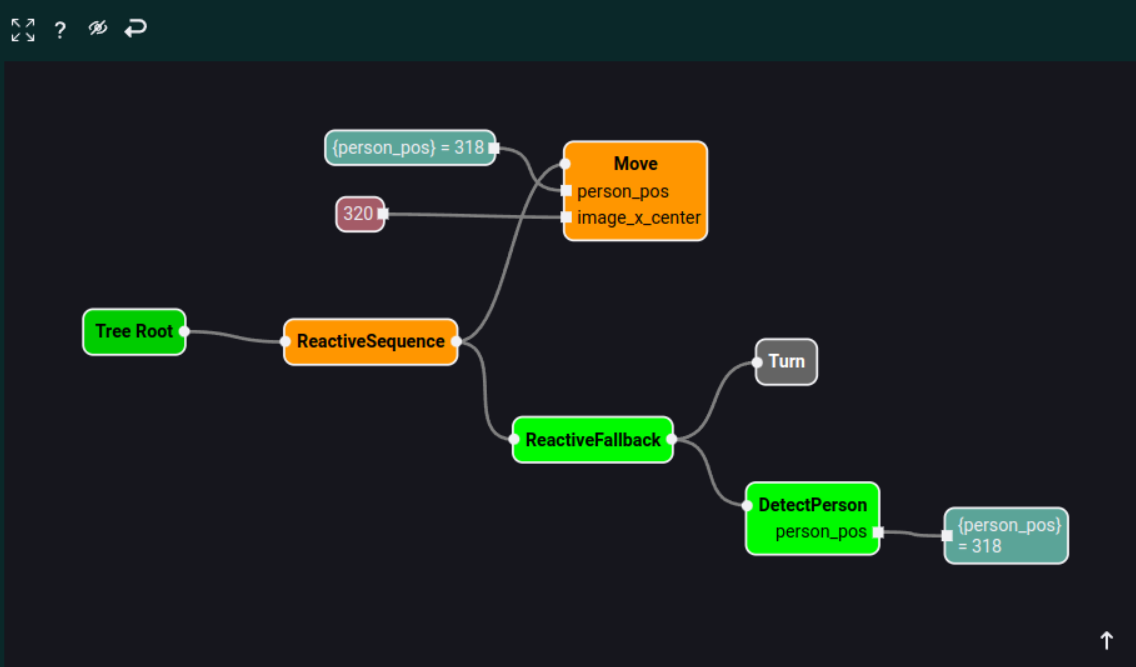
\includegraphics[width=0.8\textwidth]{figures/bt-avances/bt-monit.png}
    \caption{Apariencia del monitor de ejecución en una aplicación de ejemplo}
    \label{fig:bt-monit}
\end{figure}

Los nodos pueden mostrar cuatro estados distintos dependiendo de su ejecución:

\begin{itemize}
    \item Verde: el nodo ha acabado correctamente, devuelve \textit{Success}.
    \item Naranja: el nodo está ejecutándose, devuelve \textit{Running}.
    \item Rojo: el nodo ha fallado, devuelve \textit{Failure}.
    \item Gris: el nodo no se ejecuta.
\end{itemize}

\begin{figure}[H]
    \centering
    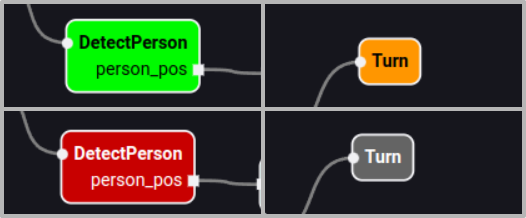
\includegraphics[width=0.5\textwidth]{figures/bt-avances/bt-monit-states.png}
    \caption{Estados de las acciones en el monitor de ejecución}
    \label{fig:bt-monit-state}
\end{figure}

Si una etiqueta tiene acceso al \textit{blackboard} esta tendrá su contenido actualizado, como se muestra en la imagen inferior.

\begin{figure}[H]
    \centering
    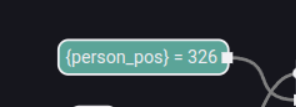
\includegraphics[width=0.5\textwidth]{figures/bt-avances/bt-tag-monit.png}
    \caption{Apariencia de una etiqueta con acceso al \textit{blackboard} en el monitor de ejecución}
    \label{fig:bt-tag-monit}
\end{figure}

\subsection{Entorno dockerizado}

Como se ha mencionado en el apartado anterior, el entorno dockerizado debe enviar el estado en el que se encuentra la aplicación en todo momento. Para conseguirlo ha hecho falta modificar el launcher de la aplicación robótica que BT Studio envía al entorno de ejecución, más detalle en la sección \ref{bt-studio:ejecutor}, para que este obtenga el estado de la aplicación, lo formatee y lo guarde en un fichero, y el RAM para que envíe a BT Studio los contenidos de ese fichero cada vez que cambie.

Lo primero se ha conseguido usando las funciones de PyTrees, \textit{py\_trees.display.ascii\_tree()} y \textit{py\_trees.display.ascii\_blackboard()}, para obtener el estado del árbol y del \textit{blackboard} respectivamente. Con estos estados, se ha definido en el fichero de Python \textit{tree\_tools}, que es usado en el lanzamiento de la aplicación, una función que traduce ese estado a un formato JSON que el frontend puede procesar. Y finalmente, con el estado traducido, este se escribe en un fichero de texto.

En la parte del RAM se ha añadido un servidor que envía el contenido del fichero usando WebSockets cuando este cambia. Estos mensajes son recibidos en BT Studio por el CommsManager que posteriormente se los entrega el monitor.

\section{Ejecución dockerizada}\label{bt-studio:ejecutor}

La última de las mejoras que afecta a la nueva funcionalidad de BT Studio es la ejecución dockerizada, que es un contenedor docker que proporciona un entorno con todas las herramientas necesarias para la visualización y ejecución de las aplicaciones. Este contenedor puede ser el Robotics Backend o el propio de BT Studio \footnote{\url{https://hub.docker.com/r/jderobot/bt-studio}} que contiene a ambos. El primero es usado cuando el web IDE no necesita ser lanzado, como en Unibotics, y el otro cuando se lanza de forma \textit{offline}.

De ahora en adelante, cuando se hable del Robotics Backend es como si fuera de ambos.

\begin{figure}[H]
    \centering
    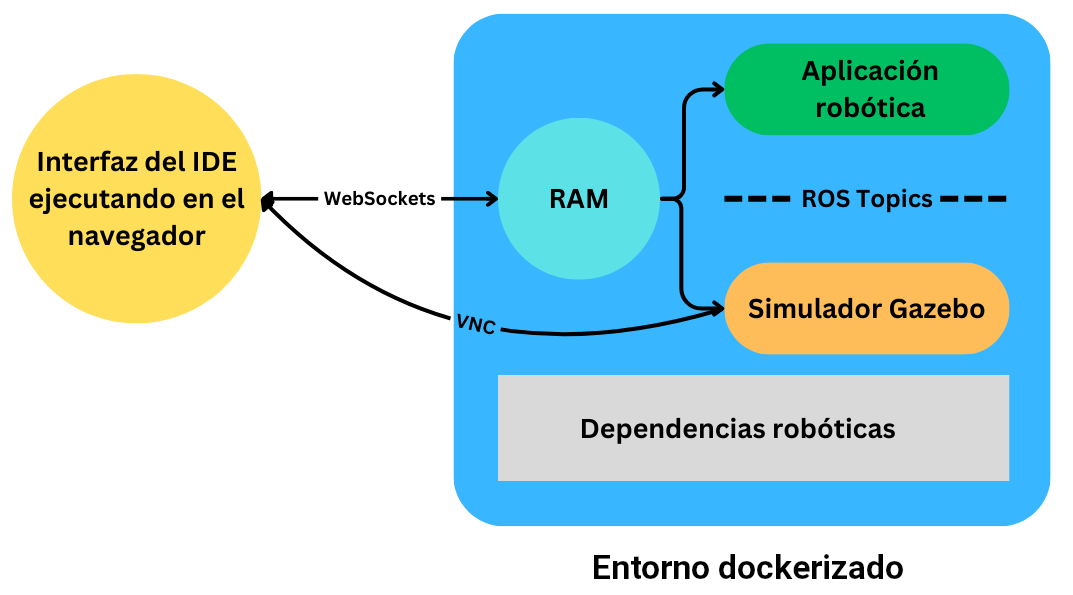
\includegraphics[width=0.8\textwidth]{figures/bt-studio/docker_exec_detail.png}
    \caption{Ejecución de una aplicación robótica con el Robotics Backend}
    \label{fig:ejemplo}
\end{figure}

\subsection{Ejecución de aplicaciones}\label{sec:conex}

Cuando se lanza BT Studio, el \textit{CommsManager} intenta conectarse al puerto 7163. Este se queda esperando hasta que se lance el Robotics Backend, ya que el RAM dentro de este arranca un servidor Websocket en ese puerto, que permite la comunicación entre ambos. Una vez conectados, se podrán enviar comandos desde el frontend web del IDE al Robotics Backend y viceversa. Esto no es solo usado a la hora de ejecutar la aplicación, sino que también se utiliza para dar funcionalidad extra el editor.

A la hora de lanzar las aplicaciones, el Robotics Backend está dividido en cuatro pasos que deben realizarse de manera secuencial y monitorizada, al igual que los escalones de una escalera (Figura \ref{fig:radi_ladder}). Estos pasos están definidos por una máquina de estados interna al RAM, que abreviaremos como \textit{manager} para que sea más sencillo entenderlo.  

Esto implica que desde el frontend web de BT Studio se deben enviar los comandos correspondientes en el orden correcto para proceder con la ejecución. De manera secuencial, los cuatro mensajes para iniciar la ejecución son estos:

\begin{enumerate}
    \item \textbf{Connect}: abre la conexión con el servidor Websocket. El estado del \textit{manager} pasa a ser \textit{connected}. Esto ocurre cuando el \textit{CommsManager} se conecta al Robotics Backend.
     
    \item \textbf{LaunchUniverse}: envía un mensaje que contiene el universo que se desea lanzar, si este es de la base de datos se envía la información que se extrae de esta, y si es personalizado se envía un ZIP con todo el universo. En este paso se lanza el simulador de Gazebo, ya sea la versión Classic o Harmonic. El estado del \textit{manager} pasa a ser \textit{universe\_ready}. 
     
    \item \textbf{PrepareVisualization}: envía un mensaje con el tipo de visualización que requiere la aplicación. En el caso de BT Studio se crean dos visores VNC, uno para el simulador y otro para el terminal. Una vez creados, estos se conectan a sus contrapartes en el frontend web para poder visualizarlos. El estado del \textit{manager} pasa a ser \textit{visualization\_ready}. 
     
    \item \textbf{RunApplication:} se envía un ZIP que contiene la aplicación robótica. El \textit{manager} lo descomprime y lanza la ejecución desde el \textit{entrypoint} que es \textit{execute\_docker.py}. El estado del \textit{manager} pasa a ser \textit{app\_ready}.
\end{enumerate}

\begin{figure}[H]
    \centering
    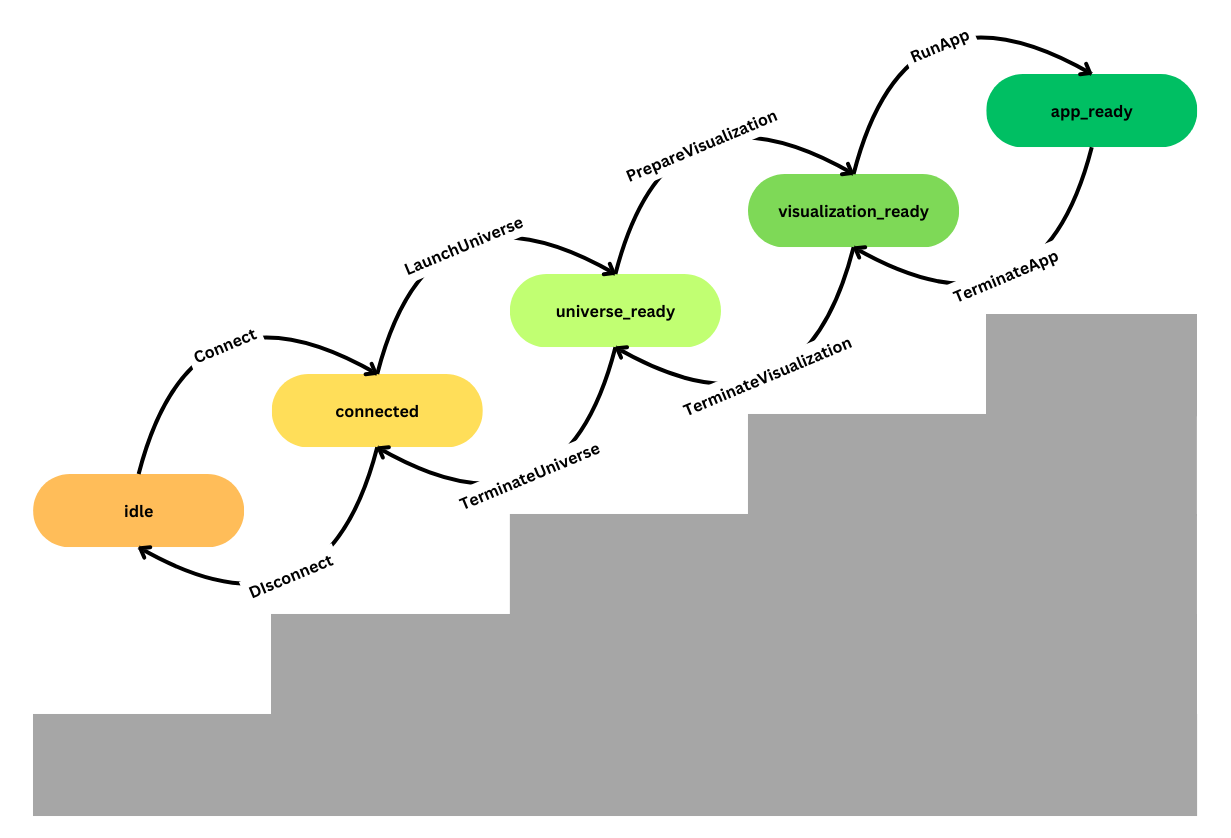
\includegraphics[width=\textwidth]{figures/bt-studio/radi_ladder.png}
    \caption{Escalera de transiciones en el Robotics Backend durante la ejecución dockerizada de una aplicación robótica}
    \label{fig:radi_ladder}
\end{figure}

Durante toda esta secuencia, el \textit{manager} ejecuta los distintos componentes como subprocesos, lo que permite almacenar el PID de cada uno para posteriormente ejecutar varias acciones. Estas pueden variar dependiendo de los distintos componentes afectados: 

\begin{itemize}
    \item \textbf{Sobre la aplicación:}
    \begin{itemize}
        \item \textbf{Pause:} suspende la ejecución del proceso.
        \item \textbf{Resume:} continúa la ejecución del proceso.
        \item \textbf{TerminateApplication:} cierra  todos los procesos asociados a la ejecución de la aplicación. Además, reinicia y pausa la simulación en Gazebo. El estado del \textit{manager} pasa de \textit{application\_ready} a \textit{visualzation\_ready}. 
    \end{itemize}

    \item \textbf{Sobre la visualización:}
    \begin{itemize}
        \item \textbf{TerminateVisualization:} cierra todos los procesos asociados a la visualización, como el servidor VNC o el servidor que devuelve el estado del árbol de comportamiento. El estado del \textit{manager} pasa de \textit{visualzation\_ready} a \textit{universe\_ready}. 
    \end{itemize}

    \item \textbf{Sobre el entorno de simulación:}
    \begin{itemize}
        \item \textbf{TerminateUniverse:} cierra todos los procesos asociados a la ejecución del universo, especialmente el servidor de Gazebo. El estado del \textit{manager} pasa de \textit{universe\_ready} a \textit{connected}. 
    \end{itemize}
    
\end{itemize}

Gracias a todo esto, BT Studio permite al usuario elegir un universo de todos los predefinidos en el Robotics Backend o uno suyo propio, crear una aplicación robótica y ejecutarla en ese universo de forma repetitiva, sencilla y sin necesidad de instalación. También dota al usuario de la capacidad de control de la ejecución, al poder pararla o reiniciarla usando los botones disponibles en la esquina superior derecha de la interfaz.

\section{Integración en Unibotics}\label{sec:bt-unib}

Para finalizar, el último objetivo y el principal de esta mejora ha sido la integración total de BT Studio en la versión online de Unibotics. Esto se ha logrado de forma escalonada a lo largo del proyecto siguiendo las siguientes etapas:

\begin{enumerate}
    \item Añadir Robotics Infrastructure como submódulo de Unibotics.
    \item Modificar el lanzamiento de BT Studio para que este sea en un contenedor Docker.
    \item Añadir la ejecución dockerizada a BT Studio.
    \item Añadir BT Studio como submódulo de Unibotics.
\end{enumerate}

Como las tres primeras ya han sido contadas anteriormente, solo se va a explicar el proceso necesario para la última.

\subsection{BT Studio como submódulo}

Unibotics está compuesto de tres despliegues distintos, como se detalla en la sección \ref{sec:unibotics}: D1, D2 y D3. Para la integración se ha trabajado la mayoría del tiempo en D1 y los detalles finales en D2.

Comenzando con la integración, el primer paso fue conseguir compilar el frontend web de Unibotics en D1 con BT Studio. Esto resulto ser bastante laborioso debido a las múltiples configuraciones que hacía falta modificar en la configuración de Webpack, ya que había conflictos a la hora de tratar el código fuente de BT Studio al estar este en TypeScript y no en JavaScript como el resto de la plataforma.

Una vez que compilaba, lo siguiente era mostrarlo en el navegador correctamente. Para conseguirlo se tuvo que crear una nueva plantilla de HTML y un fichero de JavaScript en Unibotics para reemplazar el \textit{index.js} de BT Studio y que carga el resto del web IDE. Todo esto tenía como objetivo que Django reconociera cómo cargarlo, ya que este no es capaz de acceder a los ficheros situados en el submódulo de BT Studio. 

Una vez se consiguió esto, hubo múltiples problemas por las clases de CSS, ya que Unibotics sobrescribía las propias de BT Studio. Para solucionarlo hizo falta renombrarlas, todas añadiendo \textbf{bt-} al inicio de sus nombres. 

Lo último que tuvo lugar en D1 fue la copia del backend web de BT Studio al directorio situado dentro de Unibotics donde se encontraba la carpeta con el de Robotics Academy, que había sido integrado como submódulo anteriormente. Una vez el backend situado en su sitio y funcionando correctamente con los ficheros locales, se pasó al trato de archivos en remoto.

Los proyectos robóticos del usuario en BT Studio, sus archivos, cuando está integrado en Unibotics se almacenan en la nube de Amazon. Esto requiere de esa nube ya en el uso del despliegue D2 de Unibotics que además asegura que el funcionamiento va a ser igual que en el despliegue de producción D3. Estos archivos se encuentran en un servidor corriendo Amazon Simple Storage Service (Amazon S3) que ofrece un SDK o \textit{Software Development Kit} para interactuar con ellos a través del paquete de Python \textit{boto3}. Usando esto, se han replicado varias funciones que acceden a ficheros como:

\begin{itemize}
    \item \textit{aws\_pull\_ide\_file}: devuelve el contenido de un fichero.
    \item \textit{aws\_push\_ide\_file}: guarda el contenido a un fichero o si este no existe lo crea.
    \item \textit{aws\_exists\_ide\_file}: devuelve si el fichero existe.
    \item \textit{aws\_push\_ide\_folder}: crea un directorio vacío. Como en S3 no hay directorios, lo único que hace es añadir un objeto vacío con ese nombre.
    \item \textit{aws\_delete\_ide\_file}: elimina un fichero.
    \item \textit{aws\_delete\_ide\_folder}: elimina un directorio y sus contenidos de forma recursiva.
    \item \textit{aws\_rename\_ide\_file}: renombra un fichero.
    \item \textit{aws\_rename\_ide\_folder}: renombra un directorio.
    \item \textit{aws\_get\_filenames}: devuelve un listado con los nombres de los ficheros o directorios dentro de la carpeta especificada.
    \item \textit{aws\_get\_user\_projects}: devuelve una lista con todos los proyectos de un usuario.
    \item \textit{aws\_get\_user\_project\_universes}: devuelve una lista con todos los universos de un proyecto.
    \item \textit{aws\_create\_empty\_project}: crea un proyecto vacío en el directorio correspondiente al usuario: \textit{bt\_studio/NOMBRE\_USUARIO}.
    \item \textit{aws\_delete\_project}: elimina un proyecto y todos sus contenidos.
    \item \textit{aws\_create\_bt\_docker\_universe}: crea la entrada para un universo definido en el Robotics Backend.
\end{itemize}

Todas estas funciones se añaden a las funciones que componen el backend de BT Studio acompañadas de una declaración condicional que usa el acceso normal, local, si el despliegue es D1 y el acceso con S3 si es D2 o D3.

\subsection{Funcionalidad modificada}

Ha habido varios aspectos de BT Studio que se han tenido que restringir debido al peligro que podían causar a la estabilidad de la plataforma Unibotics. Debido a que Unibotics utiliza un solo servidor, se ha intentado aliviar el coste computacional del backend web sobre este. Esto ha obligado a mover toda la creación de archivos ZIP desde el backend web al frontend web que ha afectado gravemente a estas 3 funcionalidades:

\begin{itemize}
    \item La creación de la aplicación robótica: tanto para descarga local como para la ejecución dockerizada se ha migrado toda la creación del ZIP al frontend web conservando toda la funcionalidad.
    \item Los universos personalizados: no se ha conseguido mover la creación del ZIP, lo que causa que solo esté disponible por ahora en la versión \textit{offline}.
    \item La subida de código local: no se ha conseguido migrar la descompresión del ZIP, por lo que solo está disponible en la versión \textit{offline}.
\end{itemize}